\documentclass[a4paper]{article}
\usepackage[spanish]{babel}
\usepackage[utf8]{inputenc}
\usepackage{fancyhdr}
\usepackage{charter}   % tipografia
\usepackage{graphicx}
\usepackage{makeidx}

\usepackage{float}
\usepackage{amsmath, amsthm, amssymb}
\usepackage{amsfonts}
\usepackage{sectsty}
\usepackage{wrapfig}
\usepackage{listings}
\usepackage{caption}

\usepackage{hyperref} %las entradas del índice tienen links
\hypersetup{
    colorlinks=true,
    linktoc=all,
    citecolor=black,
    filecolor=black,
    linkcolor=black,
    urlcolor=black
}

\usepackage{color} % para snipets de codigo coloreados
\usepackage{fancybox}  % para el sbox de los snipets de codigo

\definecolor{litegrey}{gray}{0.94}

% \newenvironment{sidebar}{%
% 	\begin{Sbox}\begin{minipage}{.85\textwidth}}%
% 	{\end{minipage}\end{Sbox}%
% 		\begin{center}\setlength{\fboxsep}{6pt}%
% 		\shadowbox{\TheSbox}\end{center}}
% \newenvironment{warning}{%
% 	\begin{Sbox}\begin{minipage}{.85\textwidth}\sffamily\lite\small\RaggedRight}%
% 	{\end{minipage}\end{Sbox}%
% 		\begin{center}\setlength{\fboxsep}{6pt}%
% 		\colorbox{litegrey}{\TheSbox}\end{center}}

\newenvironment{codesnippet}{%
	\begin{Sbox}\begin{minipage}{\textwidth}\sffamily\small}%
	{\end{minipage}\end{Sbox}%
		\begin{center}%
		\colorbox{litegrey}{\TheSbox}\end{center}}



\usepackage{fancyhdr}
\pagestyle{fancy}

%\renewcommand{\chaptermark}[1]{\markboth{#1}{}}
\renewcommand{\sectionmark}[1]{\markright{\thesection\ - #1}}

\fancyhf{}

\fancyhead[LO]{Sección \rightmark} % \thesection\
\fancyfoot[LO]{\small{Pablo González Alba, Nicolás Quiroz, Agustín Vaghi, Lucas Vuotto}}
\fancyfoot[RO]{\thepage}
\renewcommand{\headrulewidth}{0.5pt}
\renewcommand{\footrulewidth}{0.5pt}
\setlength{\hoffset}{-0.8in}
\setlength{\textwidth}{16cm}
%\setlength{\hoffset}{-1.1cm}
%\setlength{\textwidth}{16cm}
\setlength{\headsep}{0.5cm}
\setlength{\textheight}{25cm}
\setlength{\voffset}{-0.7in}
\setlength{\headwidth}{\textwidth}
\setlength{\headheight}{13.1pt}

\renewcommand{\baselinestretch}{1.1}  % line spacing


\usepackage{underscore}
\usepackage{caratula}
\usepackage{url}

\usepackage{color}
\usepackage{clrscode3e} % para el pseudocodigo




\begin{document}

\lstset{
  language=C++,
  backgroundcolor=\color{white},   % choose the background color
  basicstyle=\footnotesize,        % size of fonts used for the code
  breaklines=true,                 % automatic line breaking only at whitespace
  captionpos=b,                    % sets the caption-position to bottom
  commentstyle=\color{mygreen},    % comment style
  escapeinside={\%*}{*)},          % if you want to add LaTeX within your code
  keywordstyle=\color{blue},       % keyword style
  stringstyle=\color{mymauve},     % string literal style
}

\thispagestyle{empty}
\materia{Algoritmos y Estructuras de Datos III}
\submateria{Segundo Cuatrimestre de 2014}
\titulo{Trabajo Práctico III}
%\subtitulo{}
\integrante{González Alba, Pablo}{476/10}{pablo.gonzalez.alba@gmail.com}
\integrante{Quiroz, Nicol\'as}{450/11}{nquiroz@dc.uba.ar}
\integrante{Vuotto, Lucas}{385/12}{lvuotto@dc.uba.ar}

\maketitle
\newpage

\thispagestyle{empty}
\vfill
\begin{abstract}
    \vspace{0.5cm}
    \textcolor{red}{\textbf{completar!}}
\end{abstract}

\thispagestyle{empty}
\vspace{1.5cm}
\tableofcontents
\newpage



%\normalsize
\newpage
\section{Objetivos generales}
\textcolor{red}{\textbf{completar!}}



\newpage
\section{Plataforma de pruebas}
El testeo de los algoritmos implementados fue realizado, principalmente, en las máquinas del laboratorio 3 del DC. \newline
\begin{itemize}
  \item \textbf{Sistema Operativo:} Ubuntu Linux 12.04 x86_64, kernel 3.2.0-30-generic

  \item \textbf{Especificaciones del Software:} el código está implementado en \textbf{C++}, compilado con \verb|-std=c++0x|.
  Utilizamos \textbf{Bash} y \textbf{Ruby} para los scripts. Los gráficos fueron realizados con \textbf{gnuplot}.

  \item \textbf{Especificaciones del Hardware:} Intel(R) Core(TM) i5-2500K CPU @ 3.30GHz, 8GB de RAM.
\end{itemize}



\newpage
\section{Ejercicio 1: Sobre k-PMP}
\subsection{Relación entre k-PMP y el problema 3 del TP 1.}
\vspace*{0.3cm}

Una relación posible entre k-PMP y el problema 3 del TP1 podría ser que, si
k-PMP tiene una solución válida, donde el peso total sea mínimo y además el peso total de la $k$-partición sea menor o igual al umbral $M$ de peligrosidad del problema 3 del TP1, esto significa que el problema 3 del TP1 tiene solución con $k$ camiones, aunque no necesariamente sea la solución óptima a este problema.

Es decir, quizás el problema 3 del TP1 pueda resolverse utilizando menos de $k$
camiones, pero no podemos inferir esta información a partir del resultado del
k-PMP, sólo saber si funciona para $k$.


\newpage
\subsection{Relación entre k-PMP y el problema de coloreo de los vértices de
            un grafo.}
\vspace*{0.3cm}

Sea $G = (V, E)$ un grafo simple. Dado un entero $k$ y una función de peso $w$
que, dado un eje $e \in E$ le asigna a $e$ un peso \textbf{estrictamente positivo},
la relación entre el problema de $k-PMP$ y el problema de coloreo de los vértices
de un grafo puede resumirse en la ecuación siguiente:

\begin{center}
  k-PMP($G$) = $0 \iff G$ es $k$-coloreable
\end{center}

Esto vale pues, si la $k$-partición de $G$ de \textbf{peso mínimo} hallada
tiene peso $0$, significa que cada conjunto de la partición (subconjuntos de $V$)
no posee aristas \textit{intrapartición}, es decir, sus extremos no se encuentran en
un mismo conjunto, por lo tanto el peso de cada uno de estos conjuntos será
\textbf{nulo} y en consecuencia también lo será la suma total de los pesos de
las aristas \textit{intrapartición}. Si esto sucede, entonces el grafo $G$ es
$k$-coloreable, pues esto significa que $V$ puede dividirse en, a lo sumo, $k$
conjuntos, siendo $k$ la cantidad máxima de colores a utilizar, de manera que no
haya vértices adyacentes en estos conjuntos, pues el \textit{coloreo} no nos permite
utilizar colores iguales para vértices adyacentes.

De la misma forma, si el grafo $G$ es $k$-coloreable, significa que utilizando
como máximo $k$ colores podemos $colorear$ los vértices del mismo, esto implica
que $V \in G$ puede dividirse en $i$ conjuntos, con $i \in {1, \dots, k}$, siendo $i$
la cantidad de colores utilizada para colorear los vértices del grafo, de manera
que en cada uno de estos conjuntos no haya vértices adyacentes, pues los agrupamos
según el color que le fue asignado a cada vértice. Esto implica que el peso de
las aristas \textit{intrapartición} es nulo para todos los $i$ conjuntos, pues éstas no
existen, ya que las aritas presentes en $G$ no conectan vértices pertenecientes a
un mismo subconjunto de $V$. Por lo tanto, al ser el peso del conjunto $i$ nulo,
la suma de los pesos de las aristas \textit{intrapartición} será también nulo, por lo
que el peso de la $k$-partición de $G$ será nulo, por lo tanto vale que $k-PMP(G) = 0$.

Es importante destacar que la relación planteada anteriormente y expresada mediante
la ecuación descripta más arriba sólo vale si la función de peso $w$ asigna a las
aristas valores positivos, caso contrario la partición peso mínimo podría ser una
cuyo peso sea negativo, la cantidad de aristas \textit{intrapartición} podría variar y el
\textit{coloreo} del grafo $G$ necesitaría más de $k$ colores para llevarse a cabo.



\newpage
\subsection{Situaciones de la vida real que pueden modelarse con k-PMP.}
\vspace*{0.3cm}

La ciudad de \textit{Malos Ayres} se encuentra dividida en $k$ barrios, para una mejor administración. Una de las compañías encargadas de brindar servicios de telecomunicaciones (internet, telefonía, etc.), es \textit{Bad Conexion S.A.}.
La compañia debe instalar $n$ antenas en la ciudad, de manera que pueda cubrir las necesidades de conexión de la misma.

En la ciudad existe también un Ente Regulador de Telecomunicaciones (\textit{ENT}), que sanciona a las compañías cuyo servicio prestado posea una calidad por debajo del mínimo establecido por ley. Dicha calidad de servicio se mide en base al \textit{grado de conectividad global} que otorga cada compañia, el cual se calcula sumando el \textit{grado de conectividad local} asociado a cada uno de los $k$ barrios de la ciudad. \textit{Bad Conexion S.A.} encontró un hueco legal en esta disposición y decidió aprovecharse del mismo, aplicando un \textit{plan de ahorro en infraestructura}, aunque ésto tenga traiga aparejado una muy probable caída en la calidad del servicio en algunas localidades.

Para esto, decide distribuir $n$ antenas entre los $k$ barrios, de manera tal que el \textit{grado de conectividad global} alcanzado sea el mínimo que esté por encima del fijado, evitando así ser sancionada por el \textit{ENT}, pero además reduciendo costos, ya que este grado puede ser mantenido aún brindando un servicio deficiente en algunos de los sectores de la ciudad.

Vemos que es posible resolver este escenario ficticio que podría llegar a plantearse en la vida real utilizando k-PMP, si planteamos el grafo de la siguiente manera:

\begin{itemize}
\item Los $n$ nodos del grafo son las antenas a distribuir en las $k$ regiones.

\item $k$ es la cantidad de regiones/barrios en las que se divide la ciudad.

\item Dado un par de nodos $i, j$, la relación entre los mismos es simétrica, dado que lo que calcula la \textit{función de ``peso''} es el \textit{nivel de conectividad} y se aplica a la arista incidente a los mismos.
\end{itemize}

De esta forma, para calcular el ``peso'' (o nivel de conectividad) de una $k$-partición, se suman los ``pesos'' de las aristas intrapartición, obteniendo así el \textit{grado de conectividad global}. Si este grado \textit{global} se mantiene por encima del mínimo requerido, es una solución válida \textit{Bad Conexion S.A.}, pudiendo así lograr su cometido.


\newpage
\section{Ejercicio 2: Algoritmo exacto para k-PMP}
\subsection{Descripción del algoritmo implementado. Podas y estrategias.}
\vspace*{0.3cm}

El algoritmo consiste en un backtracking: recorre todos los vértices y todos
los conjuntos posibles y, recursivamente, se fija cual es mejor.

La única poda consiste en cada iteración calcular si el peso actual de
la partición es mayor al peso de la partición mínima encontrada hasta
ese momento y, de ser así, cortar la recursión.

\vspace*{0.5cm}

\textbf{Pseudocódigo del algoritmo:}

\vspace*{0.3cm}

\begin{verbatim}
exacto(grafo, cantidadDeConjuntos) {
    particion = Particion(grafo, cantidadDeConjuntos)

    si cantidadDeConjuntos >= cantidadDeVertices(grafo) {
        por cada i en 1 a cantidadDeVertices(grafo) {
            agregarVertice(particion, vertice: i, conjunto: i)
        }

        return particion
    }

    verticesPendientes : pila

    por cada vertice en vertices(grafo) {
        push(verticesPendientes, vertice)
    }

    particionMin = particion

    backtracking(particion, particionMin, verticesPendientes, infinito)

    return particionMin
}

backtracking(particion, particionMin, verticesPendientes, pesoMin) {
    vertice = pop(verticesPendientes)

    por cada conjunto en conjuntos(particion) {
        agregarVertice(conjunto, vertice)

        si vacio(verticesPendientes) {
            si peso(particion) < pesoMin {
                pesoMin = peso(particion)
                particionMin = particion
            }
        } sino si peso(particion) < pesoMin {
            backtracking(particion, particionMin, verticesPendientes, pesoMin)
        }

        sacarVertice(conjunto, vertice)
    }

    push(verticesPendientes, vertice)
}
\end{verbatim}

\newpage

\subsection{Análisis de complejidad en el peor caso.}
\vspace*{0.3cm}

En primer lugar, es necesario observar que, si $k > n$, la solución el problema
es distribuir los vértices en $n$ particiones, es decir, poner un vértice en
cada partición, obteniendo peso $0$ en total, pues no hay aristas
intrapartición. Luego, al no haber diferencia en la cantidad en la resolución
del problema si $k > n$ a si $k = n$ (salvo por la presencia de particiones
vacías), se asume $k \le n$.

Teniendo en cuenta esta observación, el algoritmo busca encontrar la
partición en $k$ subconjuntos \textit{no vacíos} los $n$ vértices del grafo,
asegurando que la sumatoria de los pesos de cada uno de los $k$ subconjuntos
sea mínima. Esto conlleva, en el peor de los casos, a buscar todos los posibles
modos de distribuir $n$ elementos distinguibles en $k$ conjunto distinguibles,
de modo tal que no haya elementos repetidos en los $k$ conjuntos. La cantidad
de particiones generadas coincide en este caso con el número de
Stirling\footnote{
\url{https://en.wikipedia.org/wiki/Stirling_numbers_of_the_second_kind}} $S(n,
k)$.

Esto se logra insertando de a uno los vértices del grafo en algún conjunto de
la $k$-partición. Por cada uno de los $k$ conjuntos, el procedimiento es el
siguiente:
\begin{itemize}
  \item se inserta en el conjunto, lo que toma $O(n)$, pues para insertar un
  vértice en un conjunto de la partición, se debe calcular el nuevo peso de
  dicho conjunto y en el peor de los casos, todos los vértices pertenecen al
  conjunto.
  \item se comprueba si quedan no quedan más vértices por agregar y, de ser
  así, si el peso de la partición actual es menor al peso de la mejor partición
  encontrada hasta el momento, se toma la partición actual como la mejor
  partición hasta el momento, realizando una copia de dicha partición, lo que
  toma $O(n)$, pues en el peor de los casos todos los vértices están
  distribuidos en los conjuntos de la $k$-partición.
  \item en caso contrario, se sigue con la recursión.
\end{itemize}

Luego, en la peor de las situaciones, la complejidad de cada paso de la
recursión es $O(n . k)$.

Esto se realiza hasta generar todas las posibles particiones en $k$ conjuntos.
Luego, la complejidad total del algoritmo es
\begin{align*}
  O(S(n, k) . n . k)
\end{align*}


\newpage \subsection{Experimentación y gráficos.}
\vspace*{0.3cm}

\subsubsection{Test algoritmo exacto}

(ver \verb|info.exacto.dat.promedio|) \medskip

Para realizar este test, se generaron aleatoriamente grafos de $n$ nodos, con  $n$ inicializado en 5 e incrementándose de a 1, hasta alcanzar 30 y $m$
(cantidad de aristas) vale $\frac{n^2}{5}$, $k$ vale $\frac{n}{3}$

Para cada instancia se toma el \textbf{valor mínimo}, medido en microsegundos, luego de \textbf{10 corridas}.

Dada una combinación de $m$, $n$ y $k$, se generaron 5 instancias aleatorias con dicha combinación y se consideró el promedio entre ellas.

\vspace*{0.5cm}

\begin{figure}[h]
  \begin{center}
    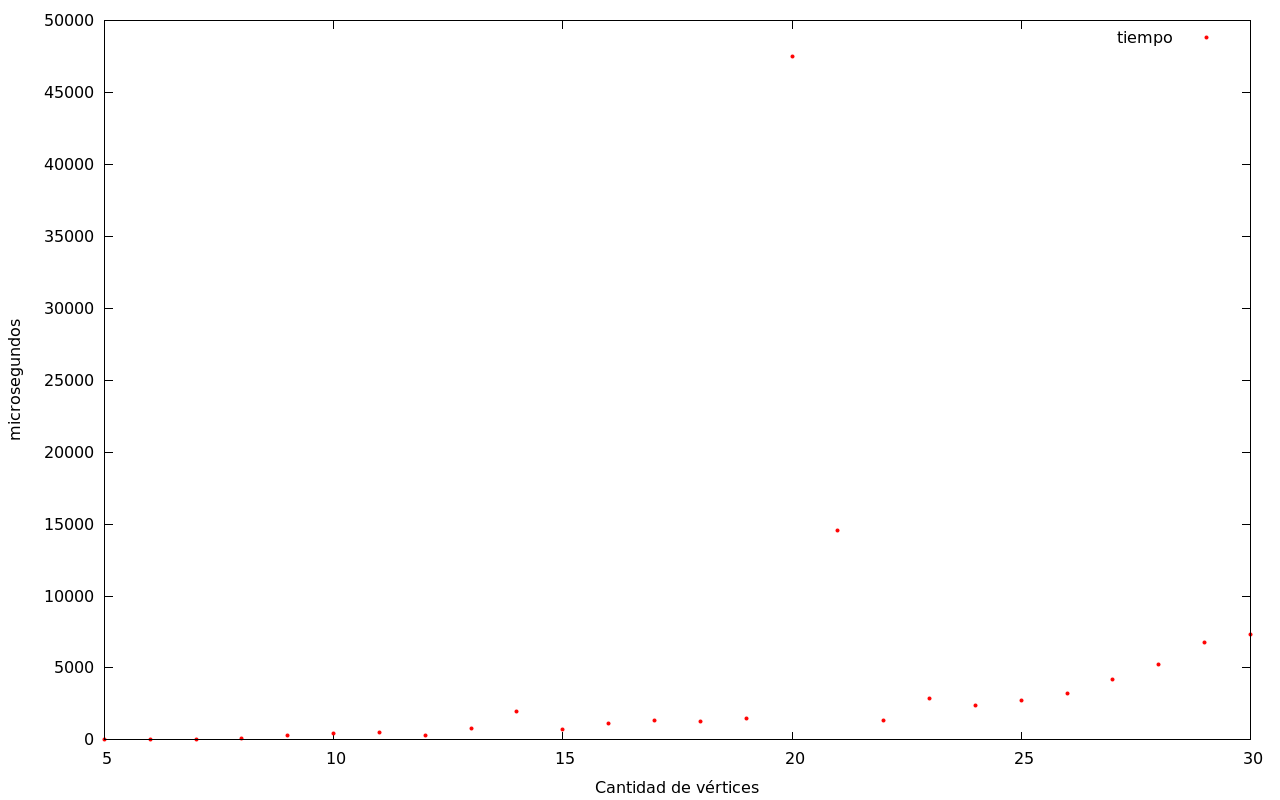
\includegraphics[scale=0.35]{imagenes/grafico-exacto.png}
  \end{center}
\end{figure}

\vspace*{0.5cm}

En el gráfico puede apreciarse que el algoritmo es \textit{``lento''}, lo cual era esperado debido a su naturaleza exponencial.


\newpage
\section{Ejercicio 3: Heurística constructiva golosa para k-PMP}
\subsection{Descripción del algoritmo implementado.}
\vspace*{0.3cm}
\textcolor{red}{\textbf{completar!}}



\newpage
\subsection{Análisis de complejidad en el peor caso.}
\vspace*{0.3cm}
\textcolor{red}{\textbf{completar!}}



\newpage
\subsection{Instancias de k-PMP para las cuales la heurística no proporciona
            una solución óptima.}
\vspace*{0.3cm}
\textcolor{red}{\textbf{completar!}}



\newpage
\subsection{Experimentación y gráficos.}
\vspace*{0.3cm}
\textcolor{red}{\textbf{completar!}}


\newpage
\section{Ejercicio 4: Heurística de búsqueda local para k-PMP}
\subsection{Descripción del algoritmo implementado.}
\vspace*{0.3cm}

La \textbf{heurística de búsqueda local} consiste en una heurística que comienza con una solución dada que intentamos mejorar. Llamaremos a esta solución ``candidata''. Luego, revisamos iterativamente sus soluciones ``vecinas''. Este conjunto de soluciones vecinas conforma el espacio de búsqueda y sus elementos son también potenciales soluciones candidatas. Esto sólo es posible si la vecindad contiene más elementos aparte de nuestra solución actual.

Si existe una mejor solución, se toma como solución actual y se repite el proceso, buscando en la vecindad de la nueva solución.

En particular, utilizamos una solución generada por la heurística golosa y verificamos mediante la búsqueda local si ésta es mejorable.

\vspace*{0.3cm}

Para nuestro algoritmo, planteamos las siguientes 2 estrategias para elegir vecindades:

\begin{itemize}
    \item \textbf{mover:} Una partición es vecina de otra si consiste en mover un único vértice de un conjunto a otro, es decir, $P$ y $Q$ son vecinas si existen $v \in A \in P$ y $B \in Q$ tales que $A - v = B$.

    \item \textbf{intercambiar:} Una partición es vecina de otra si consiste en intercambiar 2 vértices de distintos conjuntos, es decir, $P$ y $Q$ son vecinas si existen $v \in A \in P$ y $w \in B \in Q$ tales que $(A - v) \cup \{w\} = (B - w) \cup \{v\}$.
\end{itemize}

Los algoritmos consisten en, partiendo de una solución inicial, probar todas las soluciones vecinas, y continuar desde la de menor peso. Cuando no se pueda mejorar más, finaliza la ejecución.

\vspace*{0.5cm}

\textbf{Pseudocódigo con la estrategia mover:}

\vspace*{0.3cm}

\begin{verbatim}
kpmp_mover(particion) {
    pesoMin = peso(particion)
    sePuedeMejorar = true
    mientras sePuedeMejorar {
        por cada vertice en vertices(particion) {
            conjuntoDelVertice = buscarConjunto(particion, vertice)
            pesoSinVertice = peso(particion) - costo(conjuntoDelVertice, vertice)
            por cada conjunto en conjuntos(particion) excepto conjuntoDelVertice {
                peso = pesoSinVertice + costo(conjunto, vertice)
                si peso < pesoMin {
                    pesoMin = peso
                    verticeMin = vertice
                    conjuntoViejo = conjuntoDelVertice
                    conjuntoNuevo = conjunto
                }
            }
        }
        si pesoMin < peso(particion) {
            sacarVertice(conjuntoViejo, verticeMin)
            agregarVertice(conjuntoNuevo, verticeMin)
        } sino {
            sePuedeMejorar = false
        }
    }
}
\end{verbatim}

\newpage

\textbf{Pseudocódigo con la estrategia intercambiar:}

\vspace*{0.3cm}

\begin{verbatim}
kpmp_switch(particion) {
    pesoMin = peso(particion)
    sePuedeMejorar = true
    mientras sePuedeMejorar {
        por cada vertice1 en vertices(particion) {
            conjuntoDelVertice1 = buscarConjunto(particion, vertice)
            por cada vertice2 en vertices(particion) excepto que compartan conjunto {
                conjuntoDelVertice2 = buscarConjunto(particion, vertice)
                peso = peso(particion)
                    - costo(conjuntoDelVertice1, vertice1)
                    - costo(conjuntoDelVertice2, vertice2)
                    + costo(conjuntoDelVertice1, vertice2)
                    + costo(conjuntoDelVertice2, vertice1)
                si peso < pesoMin {
                    pesoMin = peso
                    verticeMin1 = vertice1
                    verticeMin2 = vertice2
                    conjuntoMin1 = conjuntoDelVertice1
                    conjuntoMin2 = conjuntoDelVertice2
                }
            }
        }
        si pesoMin < peso(particion) {
            sacarVertice(conjuntoDelVertice1, verticeMin1)
            agregarVertice(conjuntoDelVertice1, verticeMin2)
            sacarVertice(conjuntoDelVertice2, verticeMin2)
            agregarVertice(conjuntoDelVertice2, verticeMin1)
        } sino {
            sePuedeMejorar = false
        }
    }
}
\end{verbatim}



\newpage
\subsection{Análisis de complejidad del peor caso de una iteración del
            algoritmo de búsqueda local.}
\vspace*{0.3cm}

Sea $G = (V,E)$ y consideremos $n = |V|$ y $m = |E|$.

La función \texttt{buscarConjunto} recorre todos los conjuntos y en cada uno
busca, en tiempo logarítmico, el vértice dado. Esta función realiza sobre cada
conjunto $O(\log(\text{cantidad de vértices del conjunto}))$ comparaciones,
realizadas en $O(1)$. A su vez, la cantidad de elementos de cada conjunto está
acotada por $n$. Luego, la complejidad de esta función es $O(k\log(n))$, siendo
$k$ el parámetro de entrada.

\vspace*{0.3cm}

En cada iteración, el algoritmo de búsqueda local con la estrategia de
\textit{mover} comienza a recorrer cada vértice del grafo, realizando lo siguiente:
\begin{itemize}
  \item Se llama a la función \texttt{buscarConjunto}, la cual pertenece a
  $O(k\log(n))$.

  \item Por cada conjunto de la partición, se calcula el peso obtenido al
  agregarlo al conjunto, llamando a la función \texttt{costo}. Al igual que en
  la función \texttt{agregarAlDeMenosPeso} explicada en el ítem anterior, esto
  pertenece a $O(k + n)$.
\end{itemize}

Luego de recorrer cada vértice, se pueden llegar a realizar 2 llamados a
la función \texttt{costo}, que pertenece a $O(n)$.

Por lo tanto, en cada iteración del algoritmo de busqueda local, la complejidad
es $O(n (k\log(n) + k + n) + n) = O(nk\log(n) + nk + n^2 + n) = O(nk\log(n) +
n^2)$.

\vspace*{0.3cm}

En cada iteración, el algoritmo de búsqueda local con la estrategia de
intercambiar comienza a recorrer cada vértice del grafo, realizando lo siguiente:

\begin{itemize}
  \item Se llama a la función \texttt{buscarConjunto}, la cual pertenece a
  $O(k\log(n))$.

  \item Por cada uno de los otros vértices que no están en el mismo conjunto
  que el vértice actual:

  \begin{itemize}
    \item Se llama de nuevo a la función \texttt{buscarConjunto}.

    \item Se llama 4 veces a la función \texttt{costo}.
  \end{itemize}
\end{itemize}

Finalmente, se pueden llegar a realizar 4 llamados más a la función
\texttt{costo}.

Por lo tanto, en cada iteración del algoritmo de búsqueda local, la complejidad
es $O(n (k\log(n) + n (k\log(n) + k + n)) + k + n)$. Desarrollando, la
complejidad del algoritmo pertenece a $O(n^2k\log(n) + n^3)$.


\newpage \subsection{Experimentación y gráficos.}


\newpage
\section{Ejercicio 5: GRASP}
\subsection{Descripción del algoritmo implementado.}
\vspace*{0.3cm}

El algoritmo de \textbf{GRASP} consiste en utilizar una
\textit{heurística golosa aleatorizada} para obtener una primera solución
y luego ir mejorándola, aplicándole una \textit{heurística de búsqueda local}.

Esto se repite hasta llegar a un \textit{criterio de terminación} dado,
quedándose con la mejor solución encontrada hasta el momento.

\vspace{0.25cm}

El algoritmo que diseñamos utiliza el algoritmo goloso planteado en el
ejercicio 3 pero, para la selección de candidatos en la \textit{heurística
golosa aleatorizada}, se plantean 2 alternativas:

\begin{enumerate}
\item En lugar de elegir la arista más pesada, se elige una al azar de las
$X$ más pesadas.

\item En lugar de poner el vértice en el conjunto que genere el menor peso,
se elige un conjunto al azar de los $X$ que generan menor peso.
\end{enumerate}

\vspace{0.25cm}

Luego se mejora con alguno de los algoritmos de búsqueda local planteados en el ejercicio 4.

Y, finalmente, se diseñaron 2 criterios de terminación:

\begin{enumerate}
\item Elegir la mejor solución luego de $X$ iteraciones.

\item Elegir la mejor solución luego de que éste se encuentre como solución $X$
veces. Si se encuentra una solución mejor, se resetea el contador.
\end{enumerate}


Se probó con cada estrategia de la \textit{heurística golosa aleatorizada} por separado y luego con ambas. Todos estos resultados fueron probados con ambos algoritmos de localidad.

Por último también se combinaron todos con los 2 criterios de terminación, con distintos valores para las variables $X$ (independientes) detalladas anteriormente.

\vspace*{0.75cm}

\textbf{Pseudocódigo del algoritmo GRASP:}

\vspace*{0.1cm}

\begin{verbatim}
GRASP:
  Hasta que se cumpla el criterio de terminacion hacer:
    particion = heuristica golosa aleatorizada
    mejorar particion con una heuristica de busqueda local
  Devolver la mejor particion hallada
\end{verbatim}

El criterio de terminación puede ser:
\begin{itemize}
  \item Ejecutar $X$ veces.
  \item Repetir hasta que se encuentre la misma (mejor) solución $X$ veces.
\end{itemize}

\newpage
\subsection{Experimentación y gráficos.}
\vspace*{0.3cm}

Nuestro algoritmo con la meta-heurística GRASP tiene distintas variantes que
pueden modificarse. Vamos a analizar todas ellas para ver si existe una que
se comporte mejor en tiempo de ejecución y/o calidad de las soluciones.

\subsubsection{Criterio de aleatorización}

Sobre el algoritmo goloso definido en el ejercicio 3, en lugar de elegir en cada iteración la arista de mayor peso, se puede elegir una al azar de las de mayor peso. También, en lugar de guardar el vértice en el conjunto al cual le genere el menor peso total, se puede seleccionar un conjunto al azar de entre los que generen el menor peso total.

Se puede utilizar uno de esos criterios ó ambos, variando en cada
caso la cantidad de mejores elementos a seleccionar aleatoriamente.

Veamos como se comportan variando la cantidad de elementos a elegir al azar,
con un grafo de 500 vértices, con el 75\% de aristas para tener un grafo
completo y $k$ valiendo 15.
\vspace*{0.5cm}

\begin{figure}[H]
  \begin{center}
    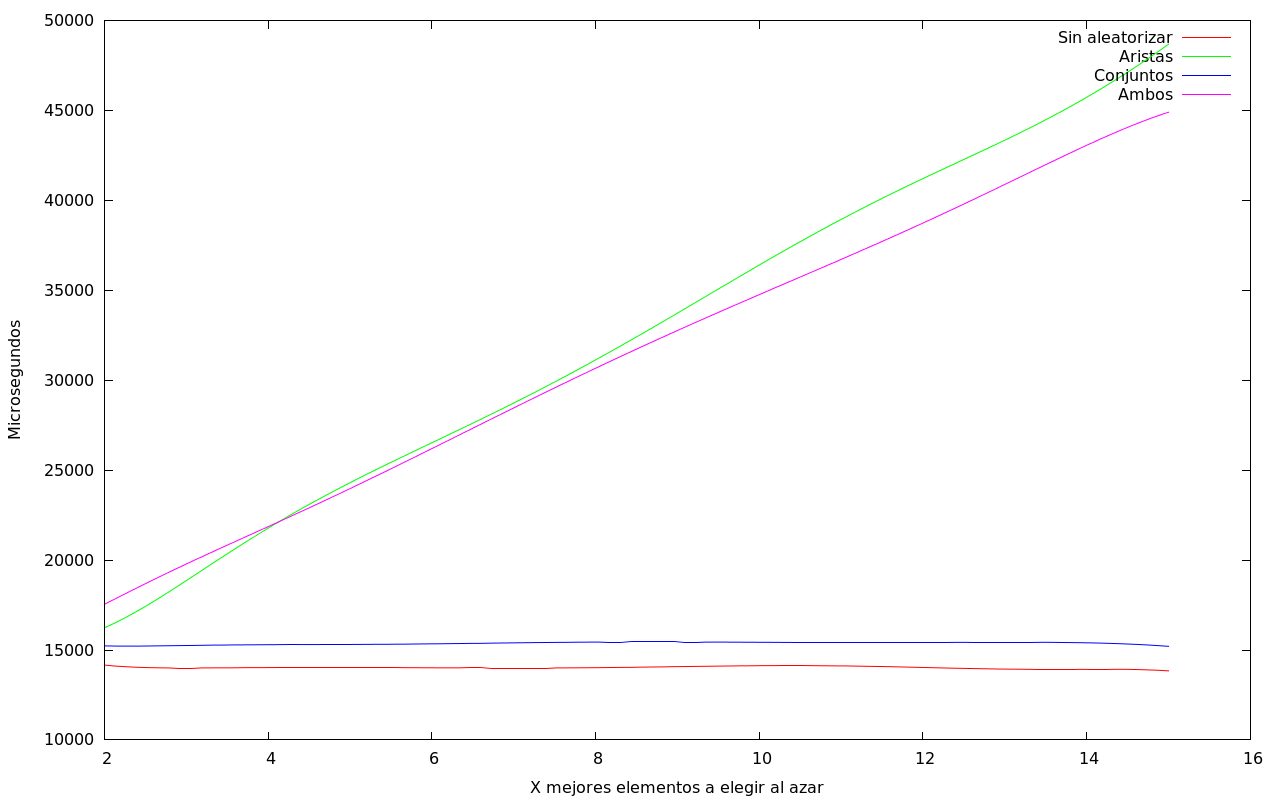
\includegraphics[scale=0.35]{imagenes/grasp-goloso-x-tiempo.png}
  \end{center}
\end{figure}

\vspace*{0.2cm}

Se puede apreciar claramente que, al aleatorizar las aristas, el tiempo crece
linealmente con respecto a la cantidad de elementos a elegir. Esto se debe
a que para elegir al azar entre los mejores, primero se están ordenando todos.

En el caso de la aristas, esto implica ordenar un conjunto de tamaño del orden
de $n^2$. En cambio, los conjuntos están fijos en 15 y ordenarlos en cada
iteración termina pareciendo constante.

Para tener en cuenta en el futuro, este comportamiento se va a mantener en
todos los casos interesantes, ya que si sabemos que van a haber casos con
$k \geq 2m$, simplemente separando todos los nodos de las $m$ aristas en 2
conjuntos distintos nos asegura un peso de 0, y se puede calcular fácilmente.

Esto suma bastante más en el caso de las aristas, ya que (en este caso)
empiezan en 375 y disminuyen de a 1. En cambio, los conjuntos están fijos en
15 y ordenar 15 en cada iteración termina pareciendo constante.

\vspace*{0.5cm}

\begin{figure}[H]
  \begin{center}
    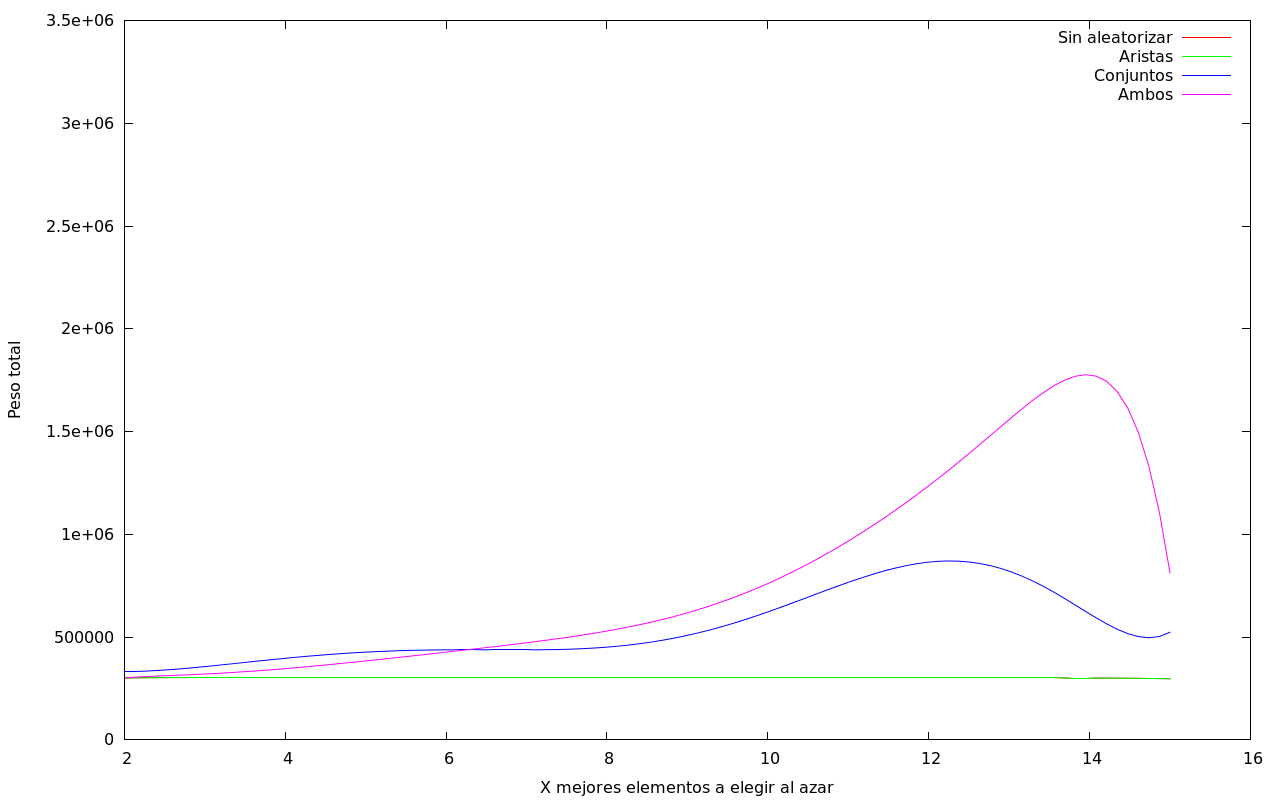
\includegraphics[scale=0.35]{imagenes/grasp-goloso-x-peso.png}
  \end{center}
\end{figure}

\vspace*{0.5cm}

Con respecto al peso, podemos ver que aumenta con respecto al goloso sin
aleatorizar cuando aumenta el $X$. Esto tiene sentido, ya que en el caso $X$
valiendo 15, con $k$ valiendo 15, el algoritmo deja de ser goloso y pasa a ser
totalmente al azar.

Lo que sí se puede observar es que aleatorizar las aristas da un resultado
apenas peor, pero despreciable con respecto a no aleatorizar nada, y no empeora
al aumentar $X$.

\vspace*{0.5cm}

\newpage Veamos si estos comportamientos se mantienen fijando $X$ en 10 (donde el peso total se mantiene relativamente acotado en todas las versiones) y modificando las otras variables.

\begin{figure}[H]
  \begin{center}
    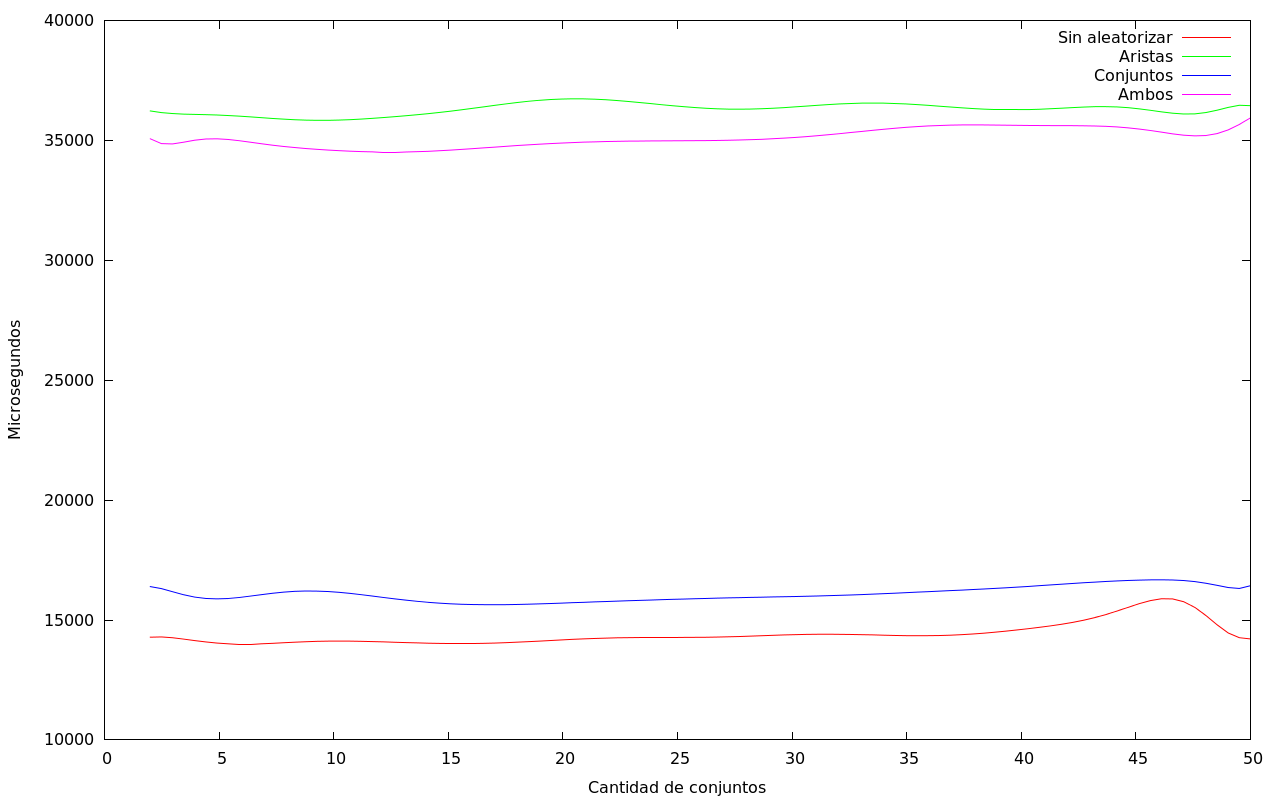
\includegraphics[scale=0.35]{imagenes/grasp-goloso-k-tiempo.png}
  \end{center}
\end{figure}

\begin{figure}[H]
  \begin{center}
    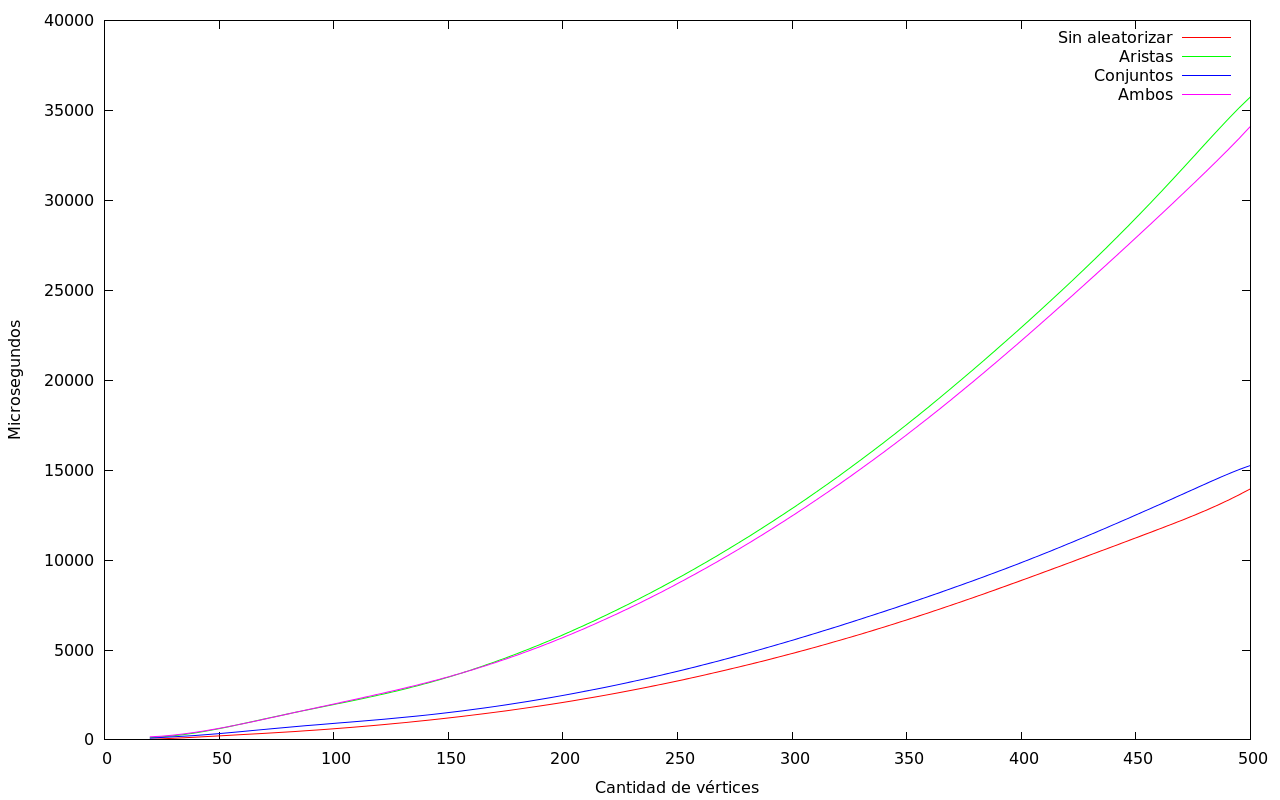
\includegraphics[scale=0.35]{imagenes/grasp-goloso-n-tiempo.png}
  \end{center}
\end{figure}

Podemos observar el mismo comportamiento, con respecto al tiempo, que veníamos
viendo. El tiempo depende de $n$ y aumenta al aleatorizar las aristas (y,
obviamente, cuando se aleatorizan ambos).

\begin{figure}[H]
  \begin{center}
    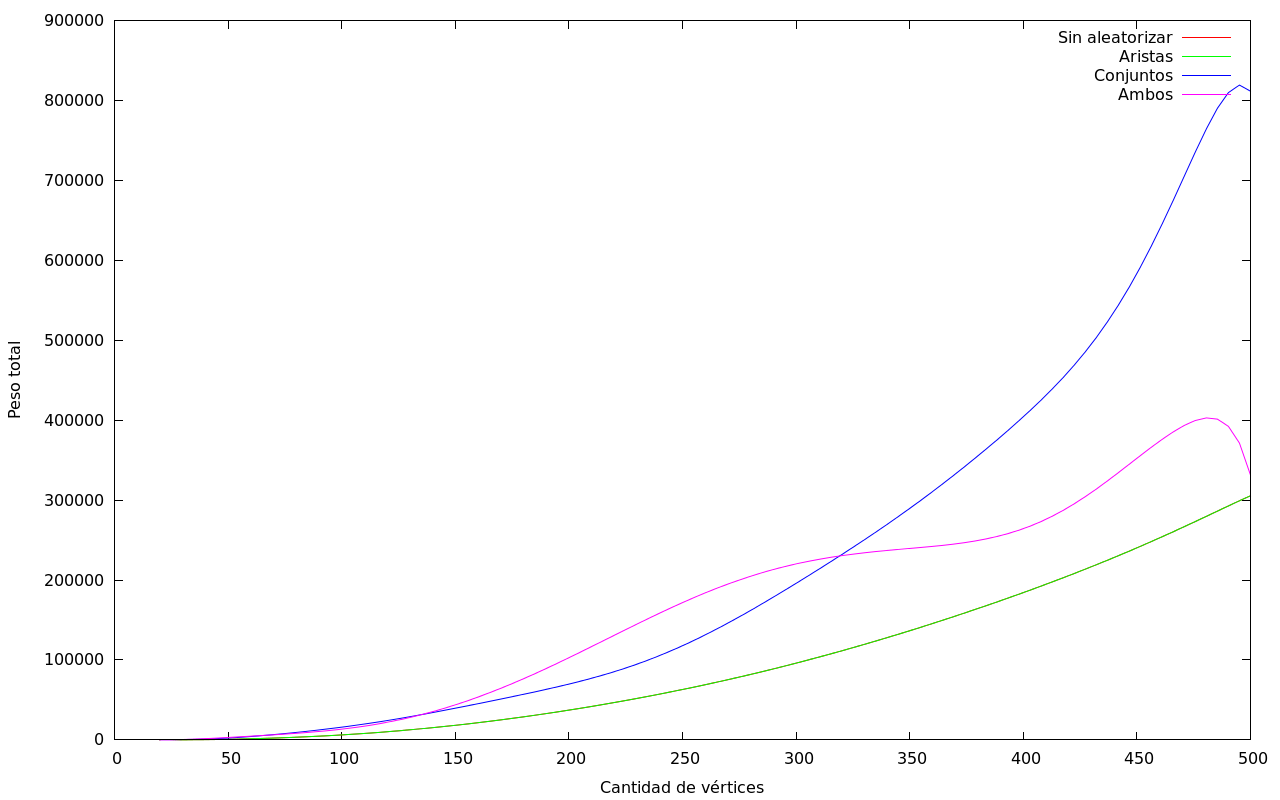
\includegraphics[scale=0.35]{imagenes/grasp-goloso-n-peso.png}
  \end{center}
\end{figure}

\begin{figure}[H]
  \begin{center}
    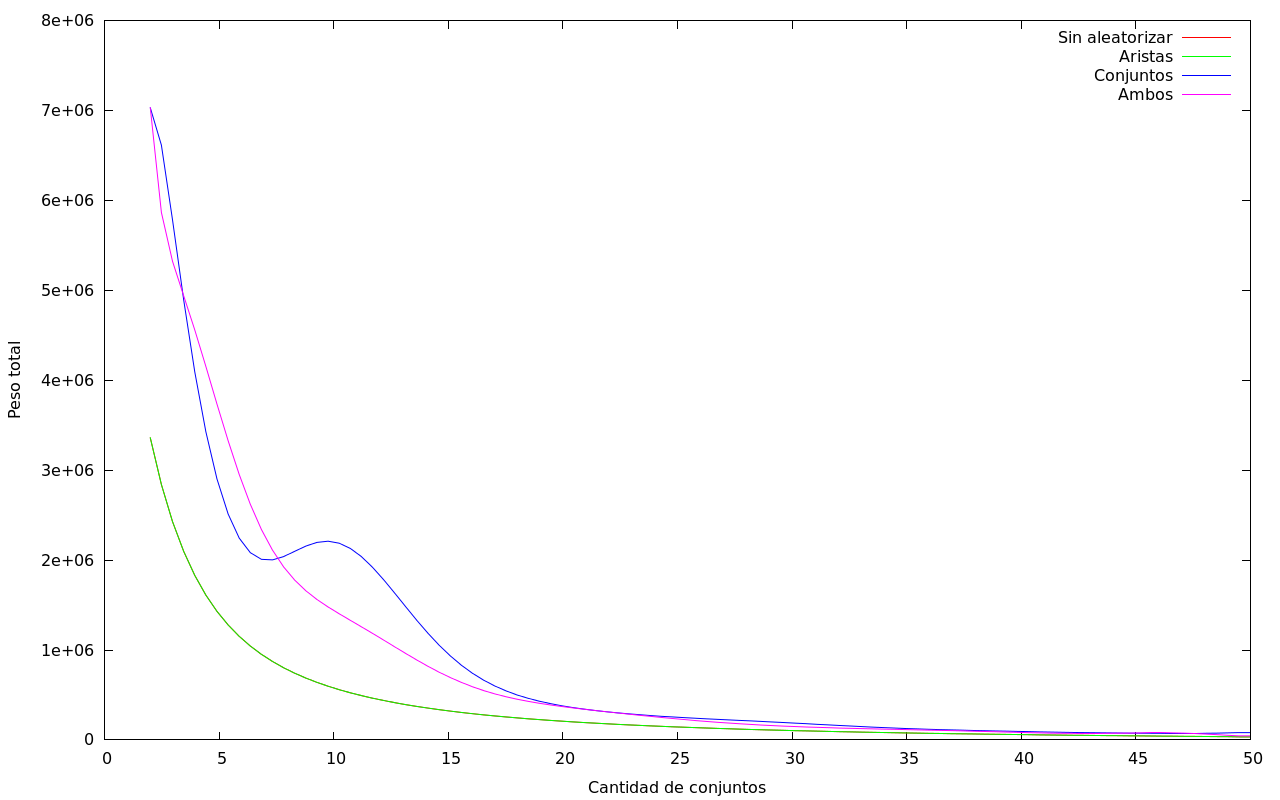
\includegraphics[scale=0.35]{imagenes/grasp-goloso-k-peso.png}
  \end{center}
\end{figure}

Con la calidad también se destacan las mismas situaciones, aleatorizar los
conjuntos genera consistentemente pesos mayores. Y aleatorizar las aristas da
resultados muy similares a no aleatorizar, dando mejores resultados en algunos
casos.

Hasta ahora todo indicaría que si se quiere priorizar tiempos se debería elegir
aleatorizar los conjuntos, pero si se prefiere calidad se debe aleatorizar las
aristas. En ningún caso conviene aleatorizar ambos, ya que sería lo peor de los
dos mundos.

\newpage \subsubsection{Junto a la heurística de búsqueda local}

Sin embargo, si el algoritmo goloso no se ejecuta solo, podría darse que una
estrategia de peores resultados por sí misma, combinada con una búsqueda local,
termine siendo mejor. Por esta razón vamos a ver los mismos casos, pero luego
de aplicarle un algoritmo de búsqueda local.

En el ejercicio identificamos que la heurística \textit{mover} se comporta
mejor que la de \textit{intercambiar}, tanto en calidad de soluciones como en
tiempo de ejecución en todos los casos. Por lo tanto utilizaremos este para las
pruebas.

Comparemos, en primer lugar, los tiempos:

\begin{figure}[H]
  \begin{center}
    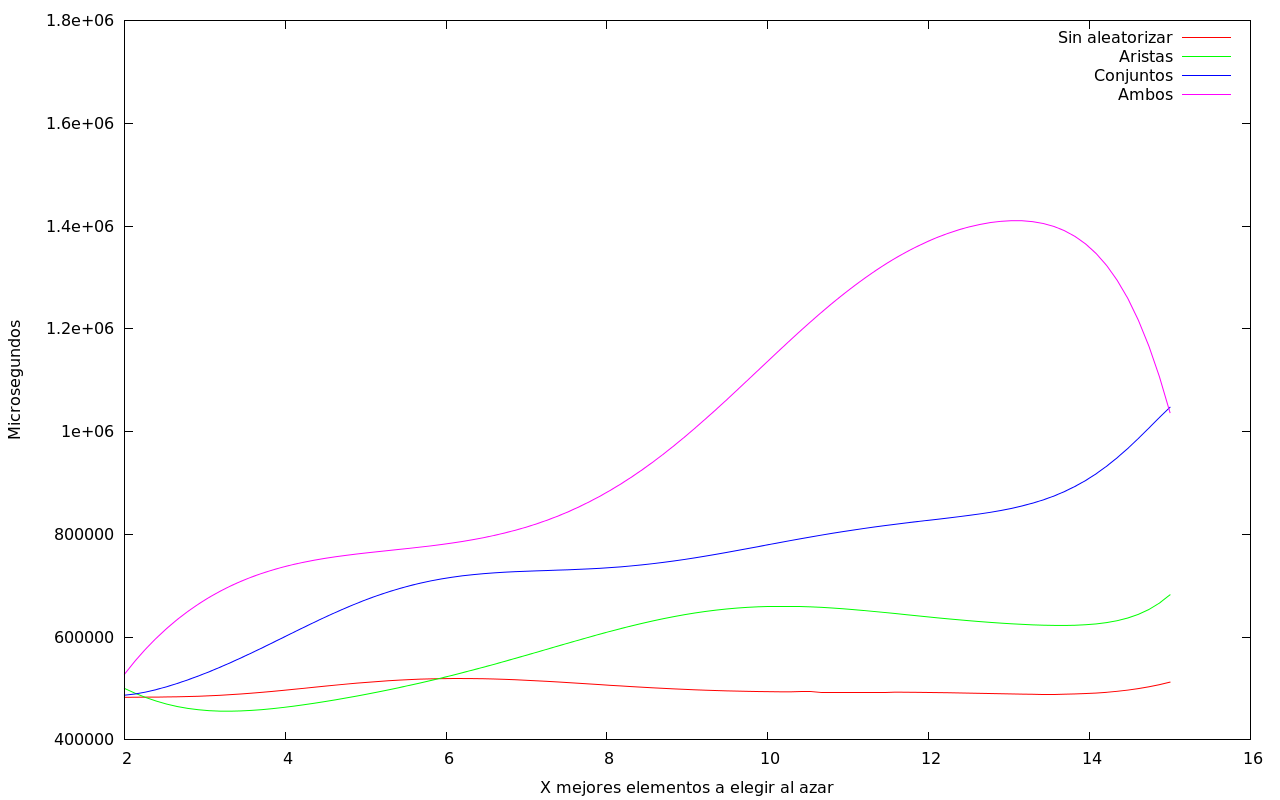
\includegraphics[scale=0.35]{imagenes/grasp-local-x-tiempo.png}
  \end{center}
\end{figure}

\begin{figure}[H]
  \begin{center}
    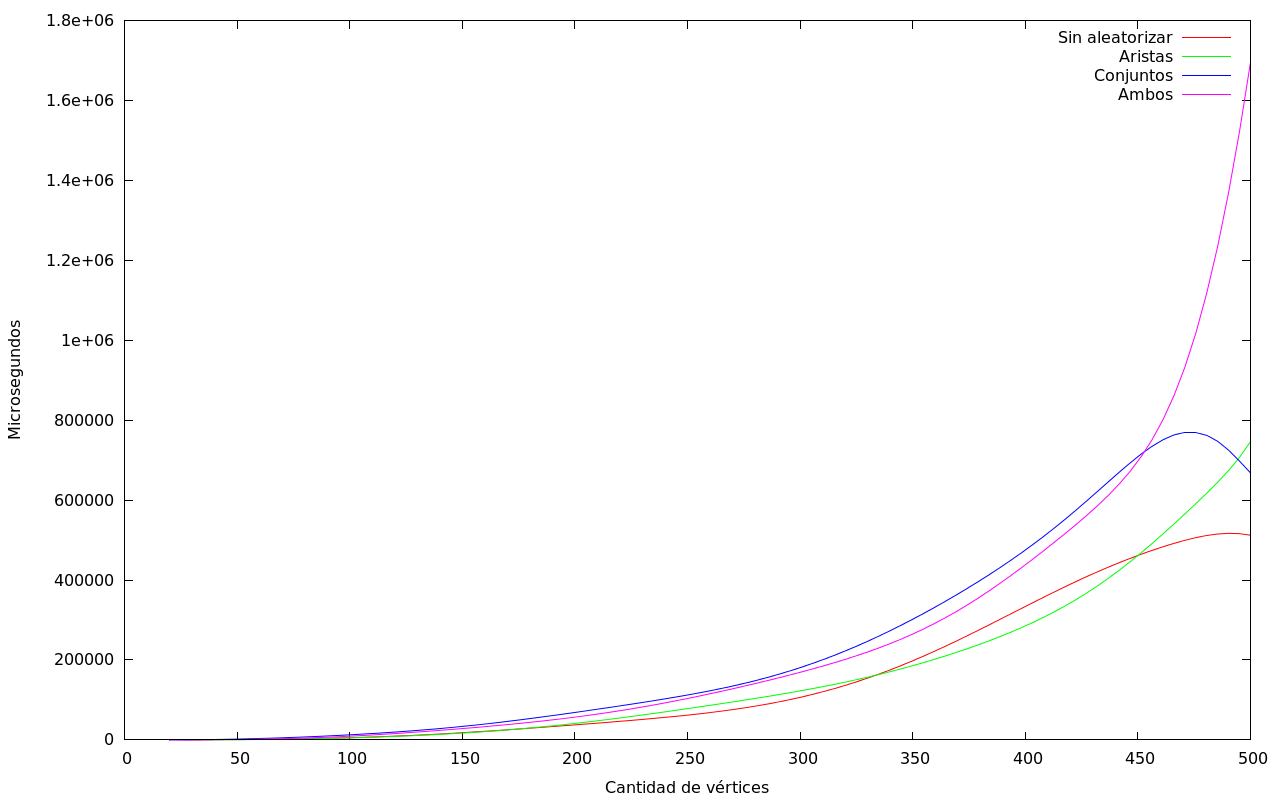
\includegraphics[scale=0.35]{imagenes/grasp-local-n-tiempo.png}
  \end{center}
\end{figure}

\begin{figure}[H]
  \begin{center}
    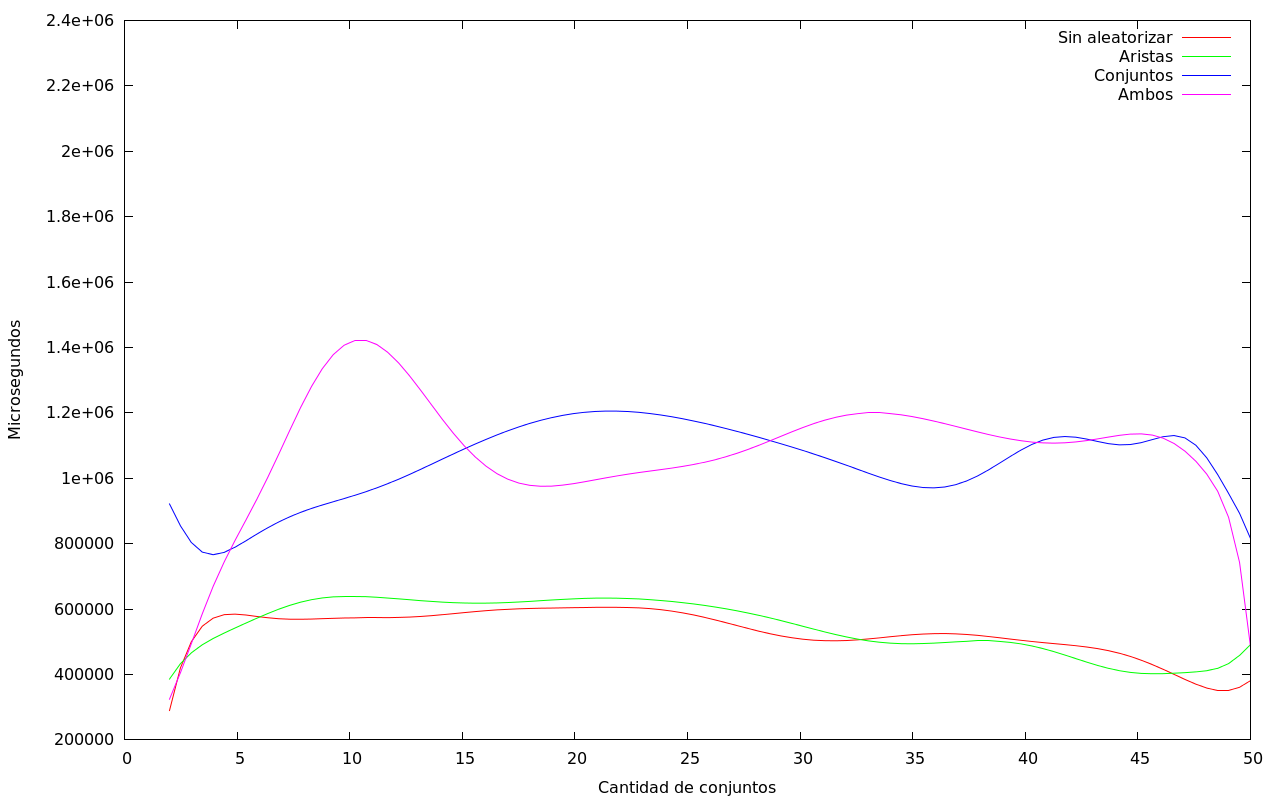
\includegraphics[scale=0.35]{imagenes/grasp-local-k-tiempo.png}
  \end{center}
\end{figure}

Estos experimentos muestran algo bastante particular: aleatorizar por aristas
es lo que menos tiempo demora, a diferencia de lo observado en la
experimentación de la búsqueda local.

En general, los tiempos de todas las versiones redujeron sus diferencias. Se
puede observar que, aunque aleatorizar las aristas sea lo más eficiente, ya no
hay una diferencia creciente entre las otras versiones del algoritmo, todas
se comportan con un orden similar.

Una explicación posible es que con una mejor versión inicial provista por
la heurística golosa, la búsqueda local demora menos en encontrar un mínimo
local.

Ahora veamos la calidad final que obtienen estos algoritmos:


\begin{figure}[H]
  \begin{center}
    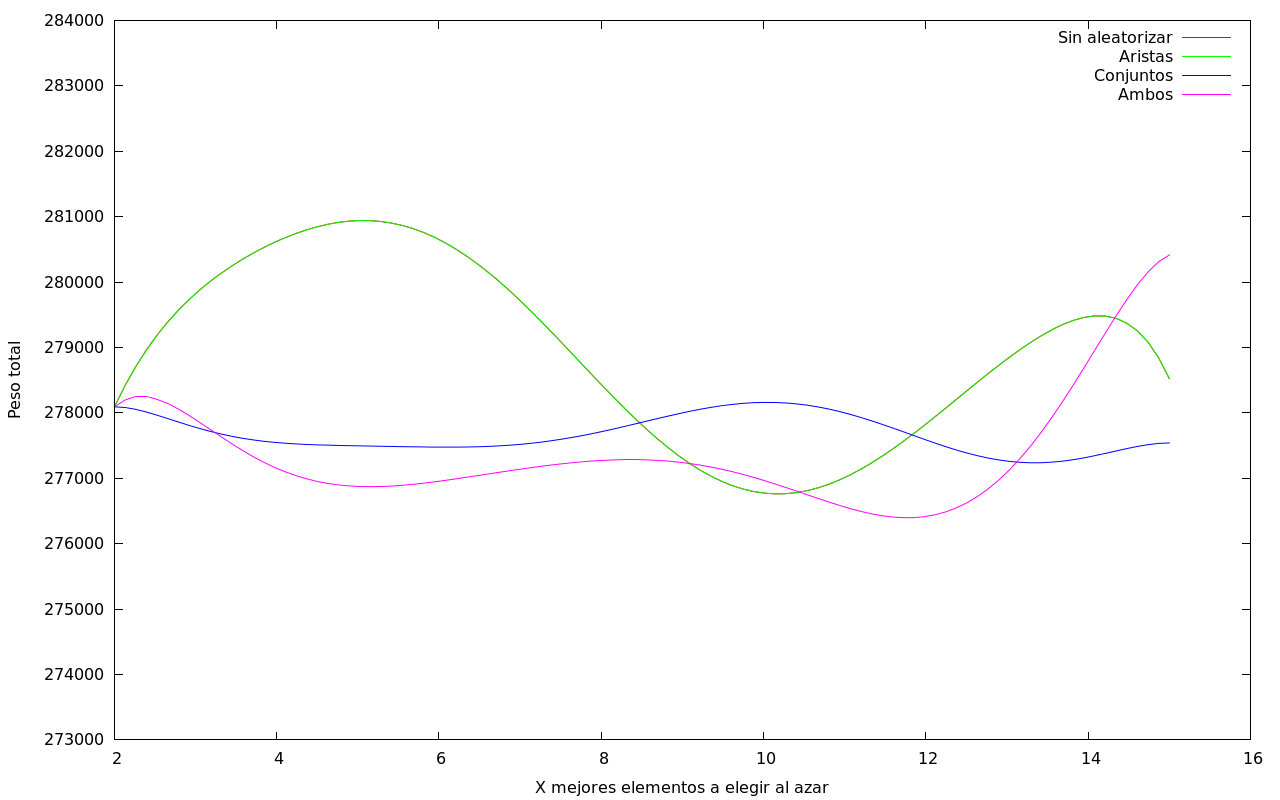
\includegraphics[scale=0.35]{imagenes/grasp-local-x-peso.png}
  \end{center}
\end{figure}

\begin{figure}[H]
  \begin{center}
    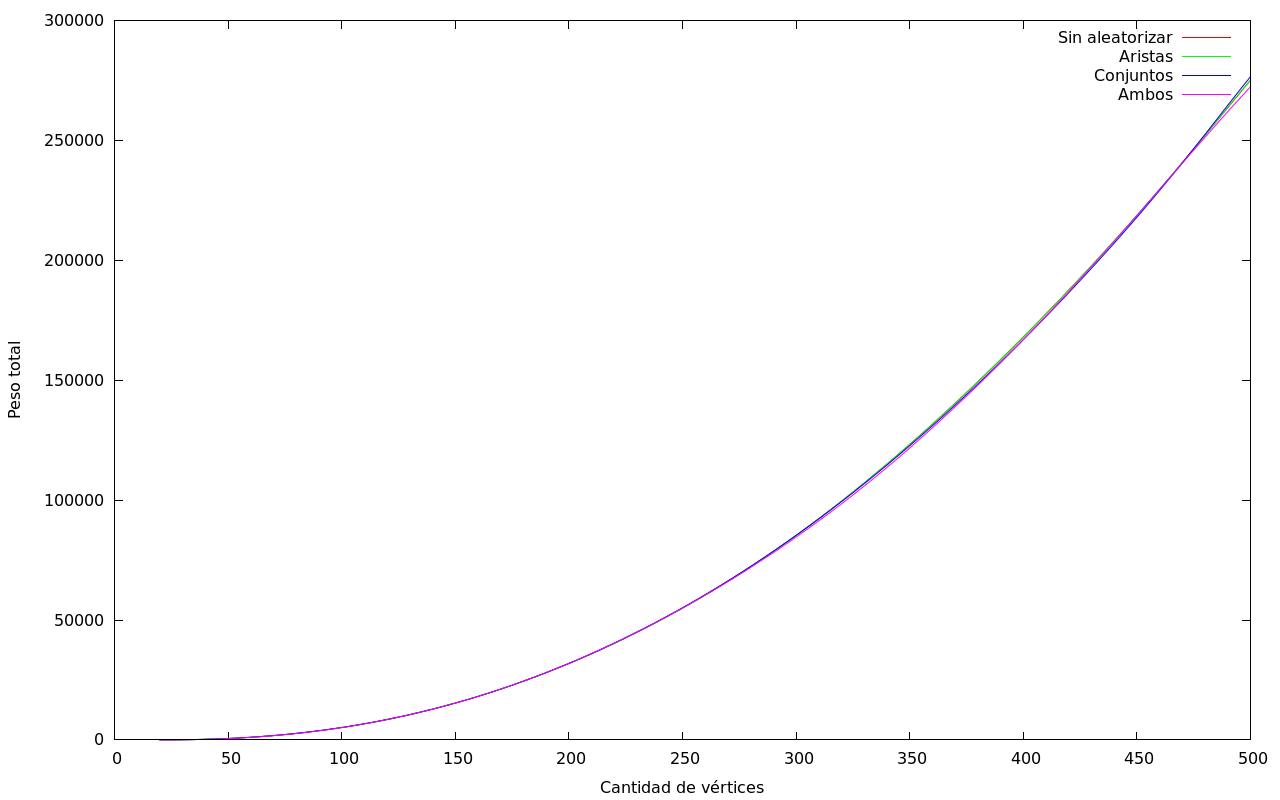
\includegraphics[scale=0.35]{imagenes/grasp-local-n-peso.png}
  \end{center}
\end{figure}

\begin{figure}[H]
  \begin{center}
    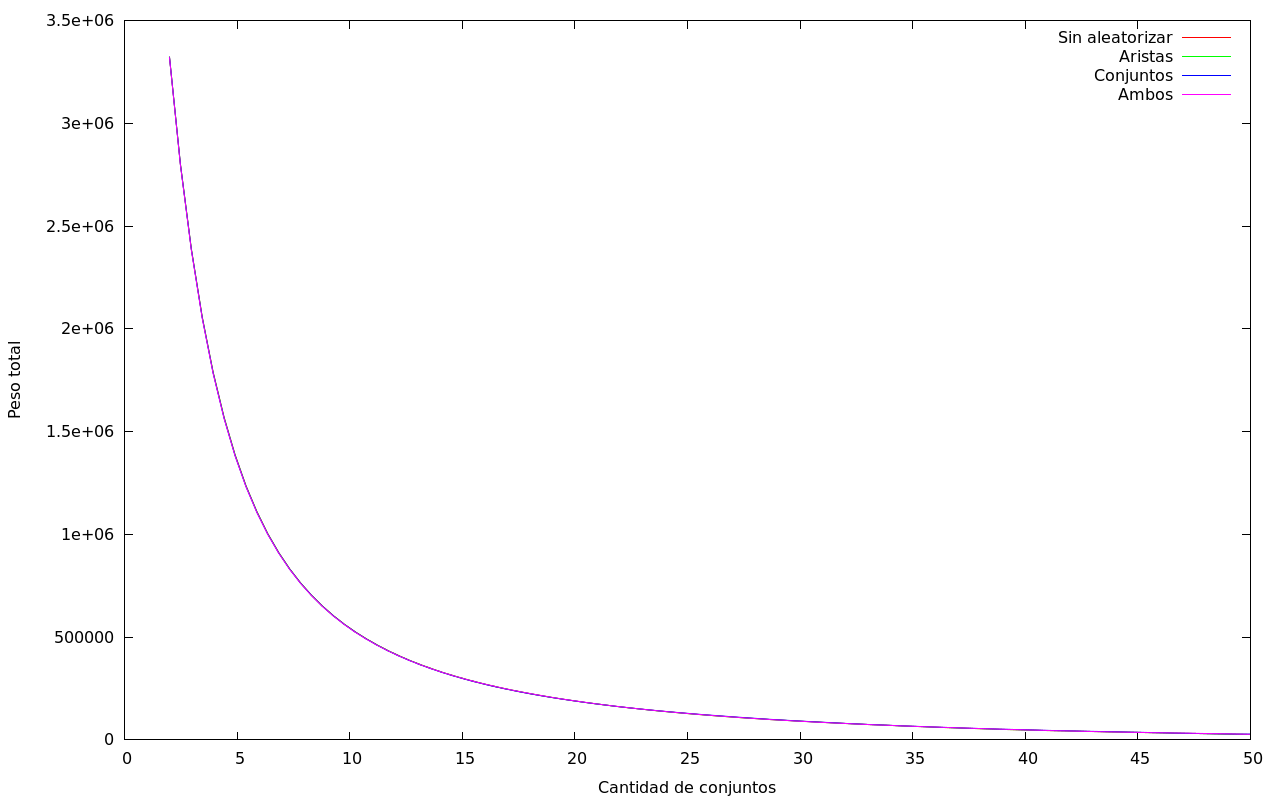
\includegraphics[scale=0.35]{imagenes/grasp-local-k-peso.png}
  \end{center}
\end{figure}

Sorprendentemente, luego de aplicar la búsqueda local, se llega a resultados
similares en todos los casos. En el gráfico que varía $X$ se puede apreciar
que, aunque no son exactamente los mismos resultados, la diferencia es casi
despreciable (menor al 1\% en la mayoría de los casos).

Combinando cualquiera de las variedades de la heurística golosa con la
búsqueda local obtenemos pesos similares, por lo que vamos a usar como
determinante el tiempo.

Consistentemente la utilización de aleatorizar únicamente las aristas dio
mejores tiempos. Por lo tanto, ésta será la utilizada. La cantidad de aristas
al azar a elegir no modifica el tiempo y apenas muy levemente el peso final.
Elegimos utilizar $X$ valiendo 10, ya que dio los mejores resultados combinando
con la búsqueda local y es un número suficientemente grande para dar variedad a
los resultados, pero no tanto que terminen siendo soluciones aleatorias.

\newpage \subsubsection{Criterio de terminación}

Para ver qué criterio de terminación conviene elegir, analizamos ambos contra
un conjunto de de 30 grafos distintos, 15 densos con 200 vértices y 15 completos
con entre 75 y 195 vértices, todos con una partición de 15 conjuntos.

Veamos como se comportan con respecto al tiempo de ejecución:

\vspace*{0.5cm}

\begin{figure}[H]
  \begin{center}
    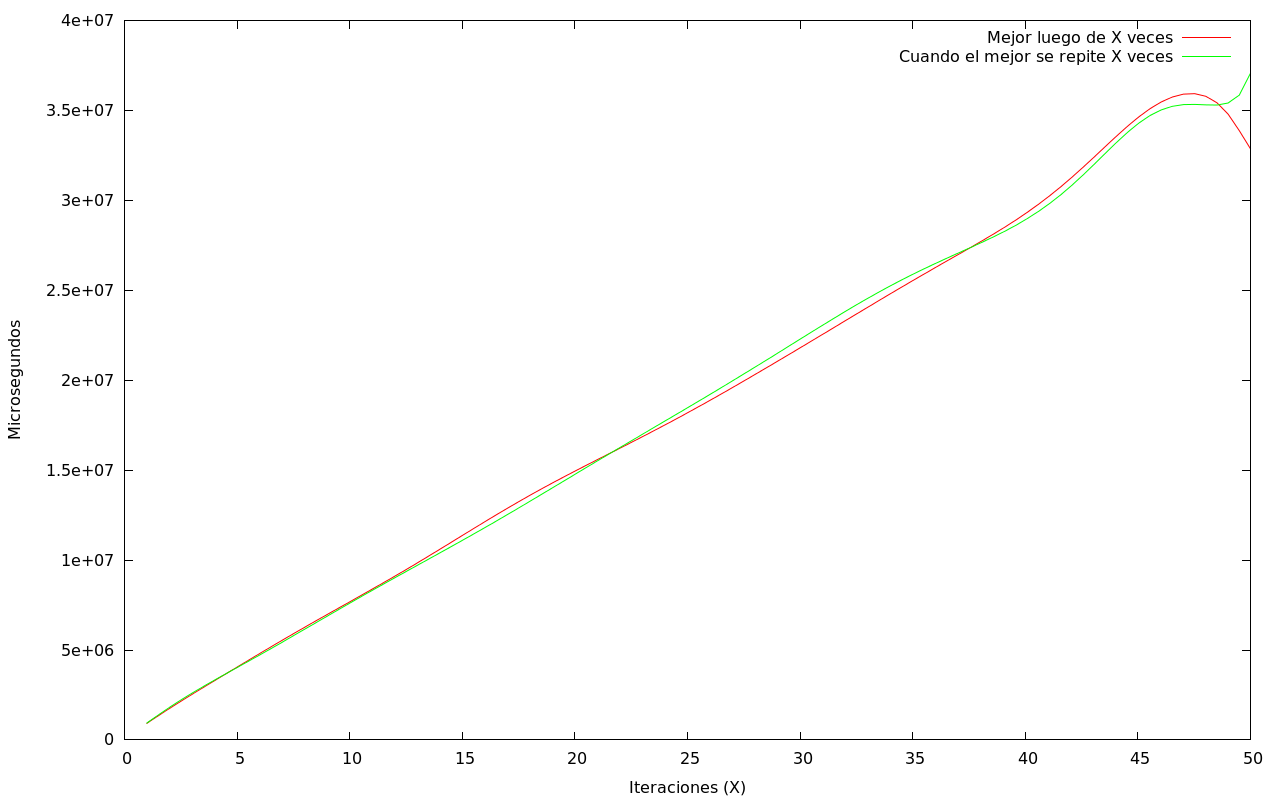
\includegraphics[scale=0.35]{imagenes/grasp-criterio-tiempo.png}
  \end{center}
\end{figure}

\vspace*{0.5cm}

Ambos tienen resultados muy similares, algo que no esperábamos, ya que uno tiene
una cantidad exacta de iteraciones y el otro podría tardar mucho más, ya que
debe encontrar la misma solución varias veces.

Esto significa que, para bien o para mal, está llegando a una misma solución
consistentemente, a pesar de la aleatorización.

Veamos entonces los pesos de las soluciones encontradas:

\vspace*{0.5cm}

\begin{figure}[H]
  \begin{center}
    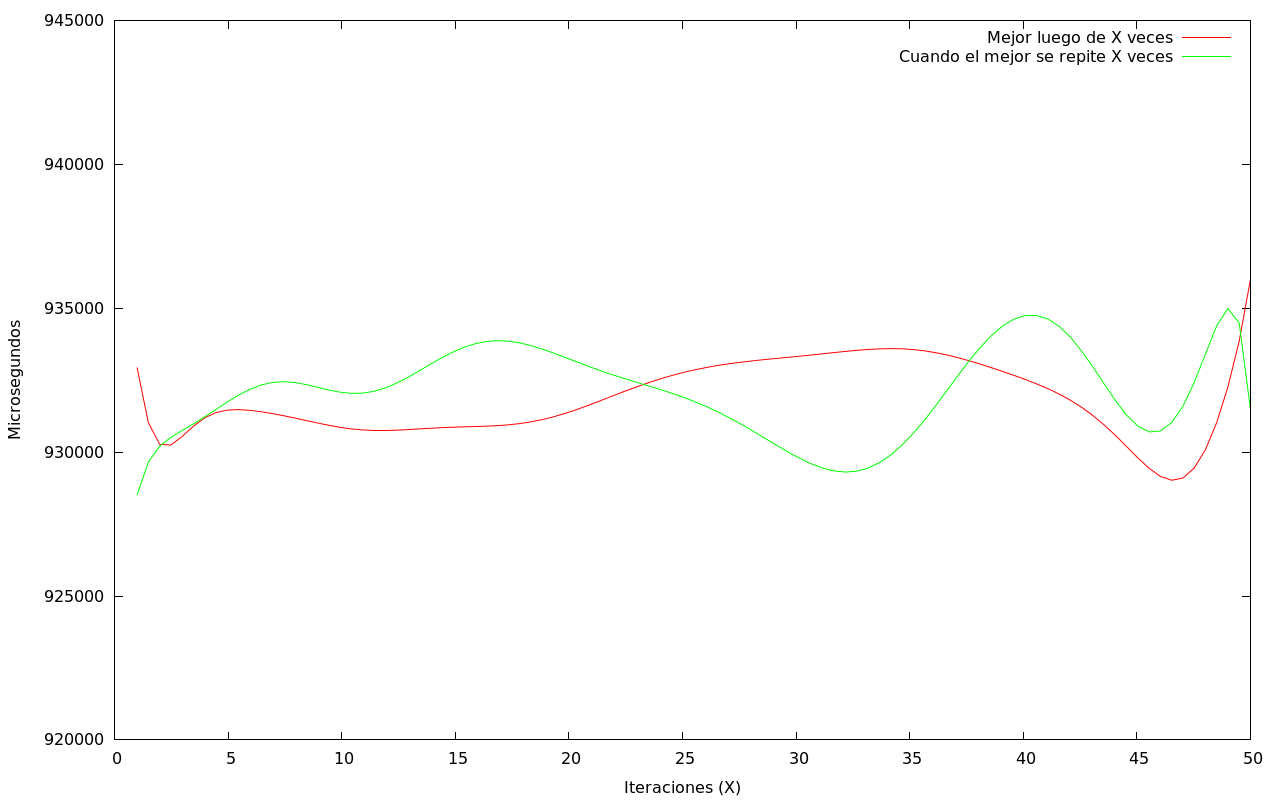
\includegraphics[scale=0.35]{imagenes/grasp-criterio-peso.png}
  \end{center}
\end{figure}

\vspace*{0.5cm}

Analizando estos resultados, no parece haber mucha diferencia, ambos tienen
resultados muy similares. Tampoco parecen reducir mucho el peso al
aumentar las repeticiones.

Elegimos quedarnos con el criterio de cuando el mejor se repita $X$ veces, con
$X = 34$, y con el criterio de parar luego de X veces con $X = 47$, siendo que
ambos dieron los mejores resultados, pero no es evidente que uno sea mejor que
el otro.


\newpage
\section{Ejercicio 6: Experimentación general y comparativa de todos los
         métodos implementados}
\subsection{Implementación elegida}

Elegimos utilizar la meta-heurística GRASP con el algoritmo goloso aleatorizado
en la elección de aristas, eligiendo al azar una de las 10 más pesadas en cada
iteración.

Luego aplicándole el algoritmo de búsqueda local que denominamos $mover$, que
define como vecindades a todas las particiones que difieren de la actual por
tener un único vértice en un conjunto distinto.

Finalmente veremos los dos criterios de terminación:
\begin{itemize}
  \item repitiendo hasta que la mejor solución se encuentre 34 veces.
  \item repitiendo exactamente 47 veces y quedándonos con la mejor hasta el momento.
\end{itemize}

\subsection{Otras implementaciones para contrastar}

Vamos a contrastar los resultados contra las siguientes implementaciones:

\begin{itemize}
  \item Exacto (mientras el tiempo de ejecución sea menor a 5 minutos)

  \item Goloso sin aleatorizar

  \item GRASP, pero aleatorizando tanto aristas como conjuntos

  \item GRASP, pero utilizando el algoritmo de búsqueda local $intercambiar$
\end{itemize}

\subsection{Experimentación}

Experimentamos con distintos tipos de grafos, variando la cantidad de vértices,
variando la cantidad de aristas según el grafo, con dos cantidades de conjuntos
distintas y, para cada combinación de valores, generar 15 grafos distintos.

Analicemos primero los tiempos:

Arbol, k=3
\vspace*{0.5cm}

\begin{figure}[h]
  \begin{center}
    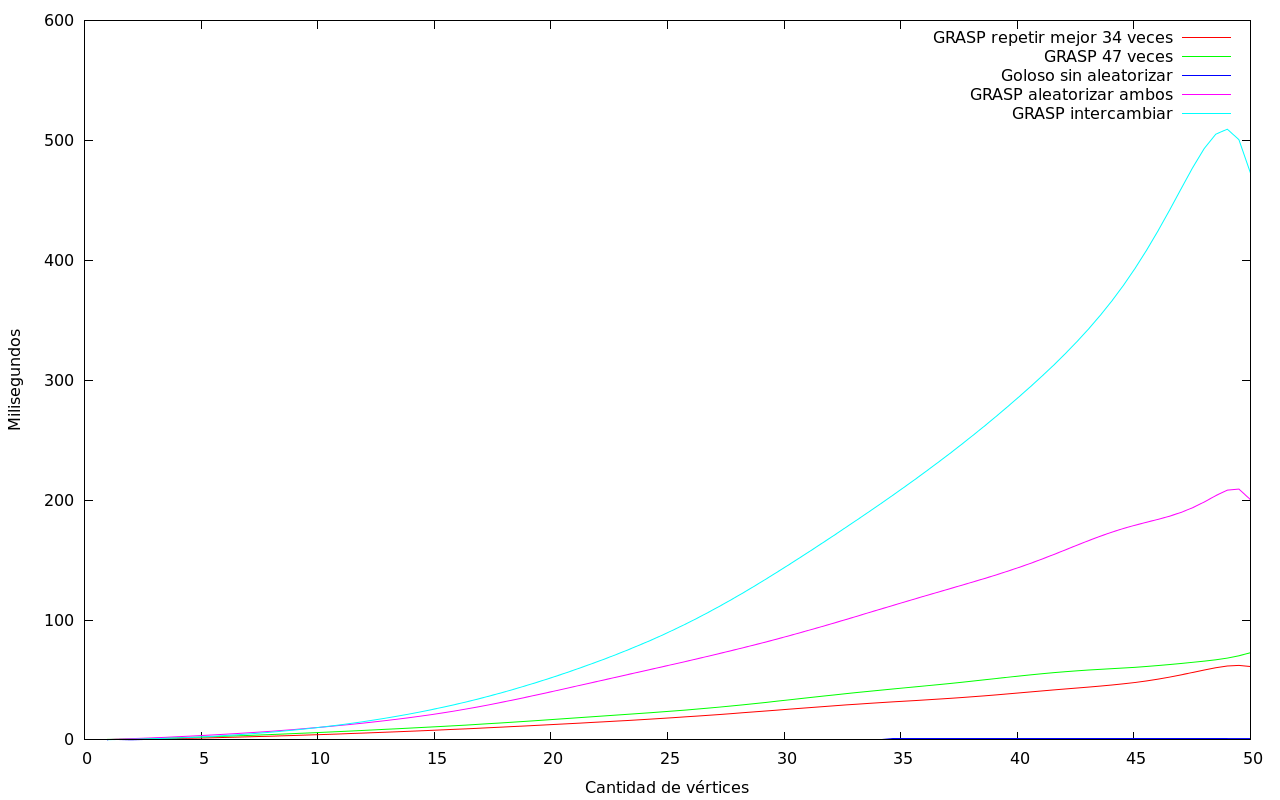
\includegraphics[scale=0.35]{imagenes/ej6-arbol-k3-tiempo.png}
  \end{center}
\end{figure}

\vspace*{0.5cm}

Arbol, k=7
\vspace*{0.5cm}

\begin{figure}[h]
  \begin{center}
    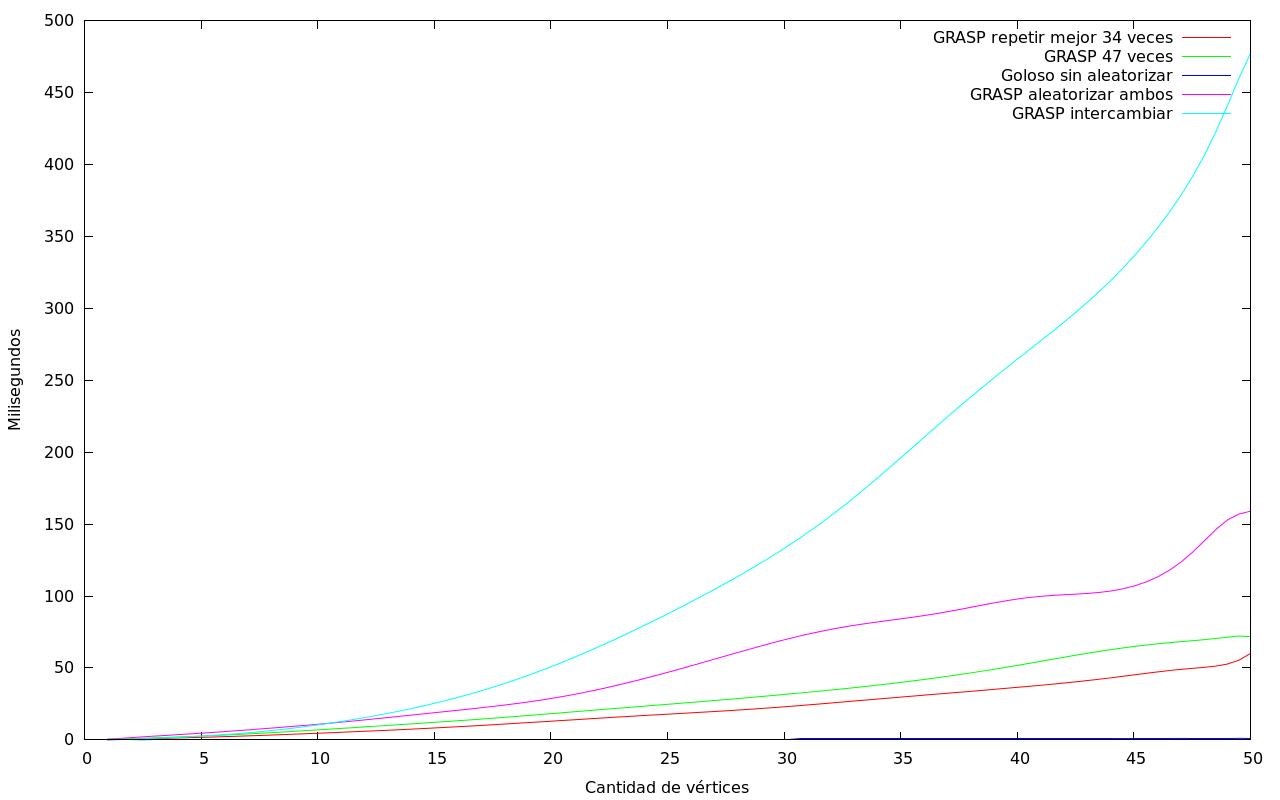
\includegraphics[scale=0.35]{imagenes/ej6-arbol-k7-tiempo.png}
  \end{center}
\end{figure}

\vspace*{0.5cm}

Completo, k=3
\vspace*{0.5cm}

\begin{figure}[h]
  \begin{center}
    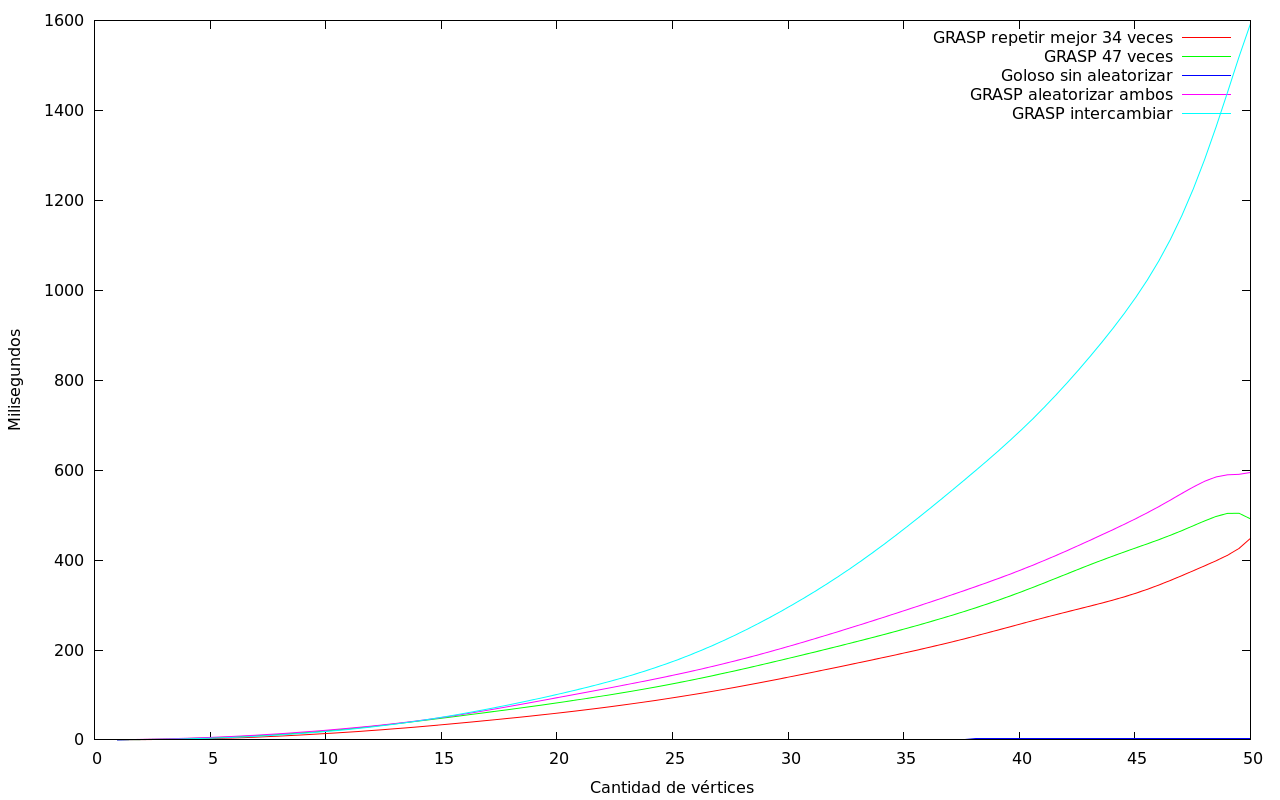
\includegraphics[scale=0.35]{imagenes/ej6-completo-k3-tiempo.png}
  \end{center}
\end{figure}

\vspace*{0.5cm}

Completo, k=7
\vspace*{0.5cm}

\begin{figure}[h]
  \begin{center}
    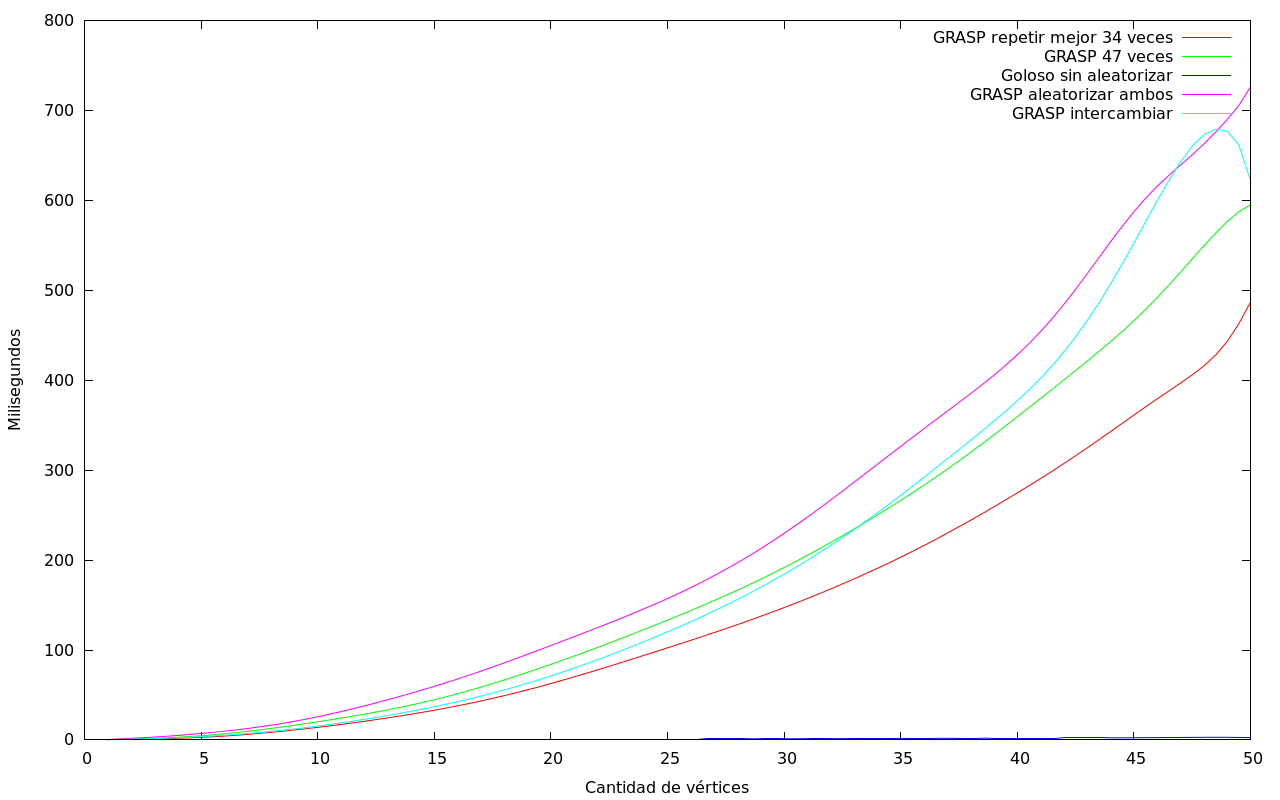
\includegraphics[scale=0.35]{imagenes/ej6-completo-k7-tiempo.png}
  \end{center}
\end{figure}

\vspace*{0.5cm}

Denso, aristas con pesos iguales, k=3
\vspace*{0.5cm}

\begin{figure}[h]
  \begin{center}
    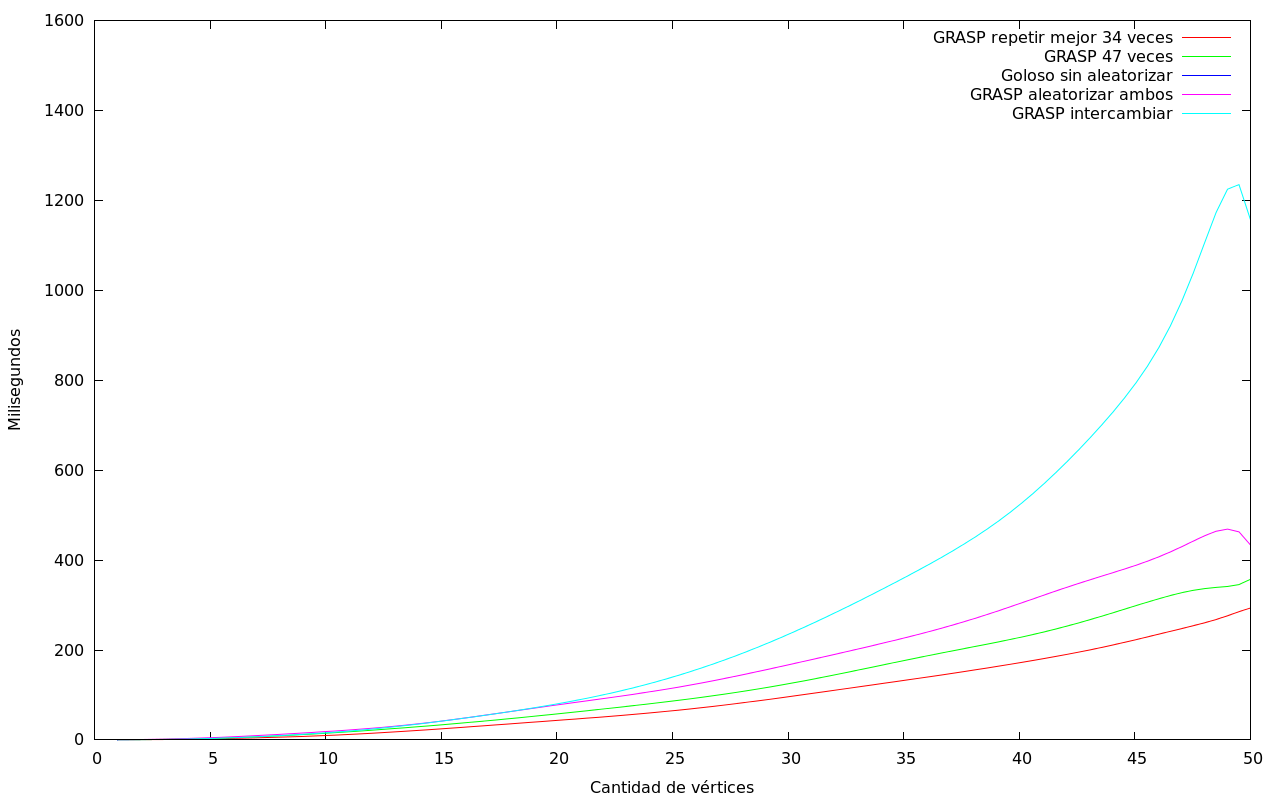
\includegraphics[scale=0.35]{imagenes/ej6-denso-pesos-iguales-k3-tiempo.png}
  \end{center}
\end{figure}

\vspace*{0.5cm}

Denso, aristas con pesos iguales, k=7
\vspace*{0.5cm}

\begin{figure}[h]
  \begin{center}
    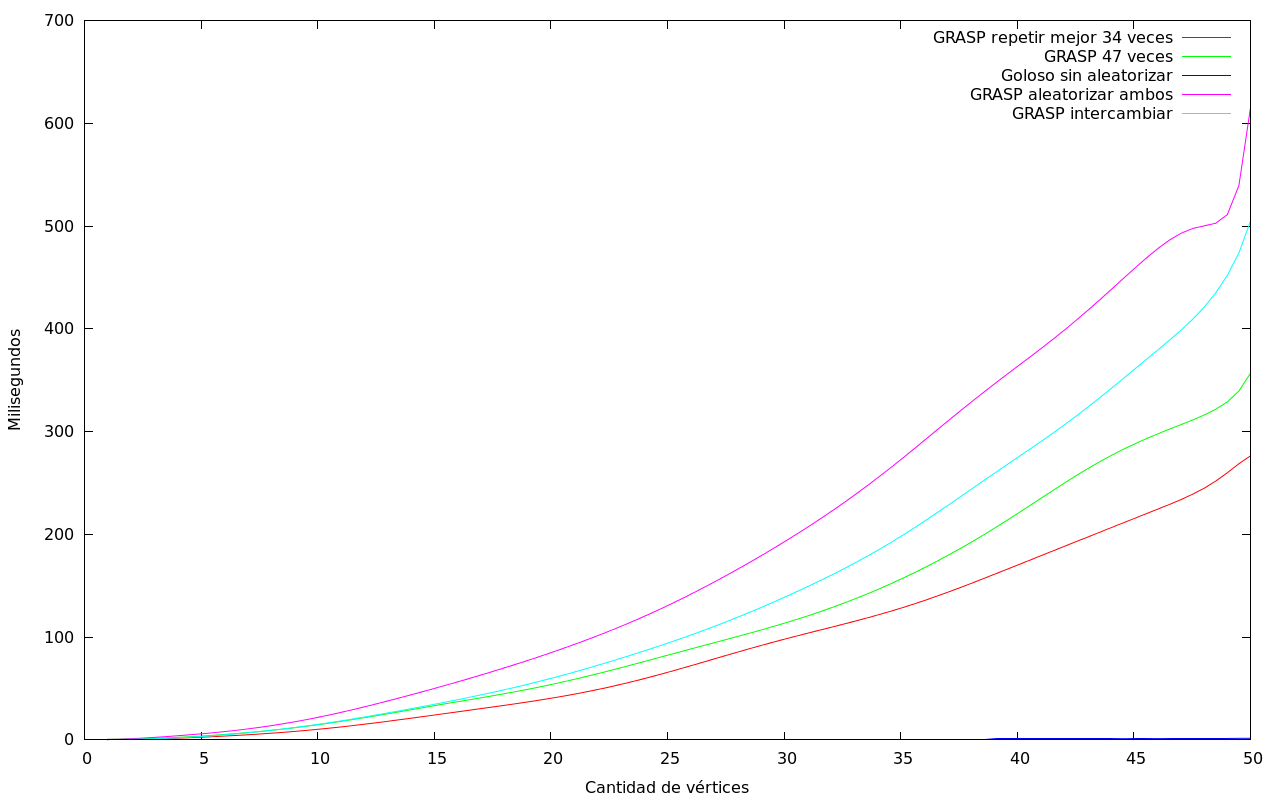
\includegraphics[scale=0.35]{imagenes/ej6-denso-pesos-iguales-k7-tiempo.png}
  \end{center}
\end{figure}

\vspace*{0.5cm}

Denso, aristas con pesos distintos, k=3
\vspace*{0.5cm}

\begin{figure}[h]
  \begin{center}
    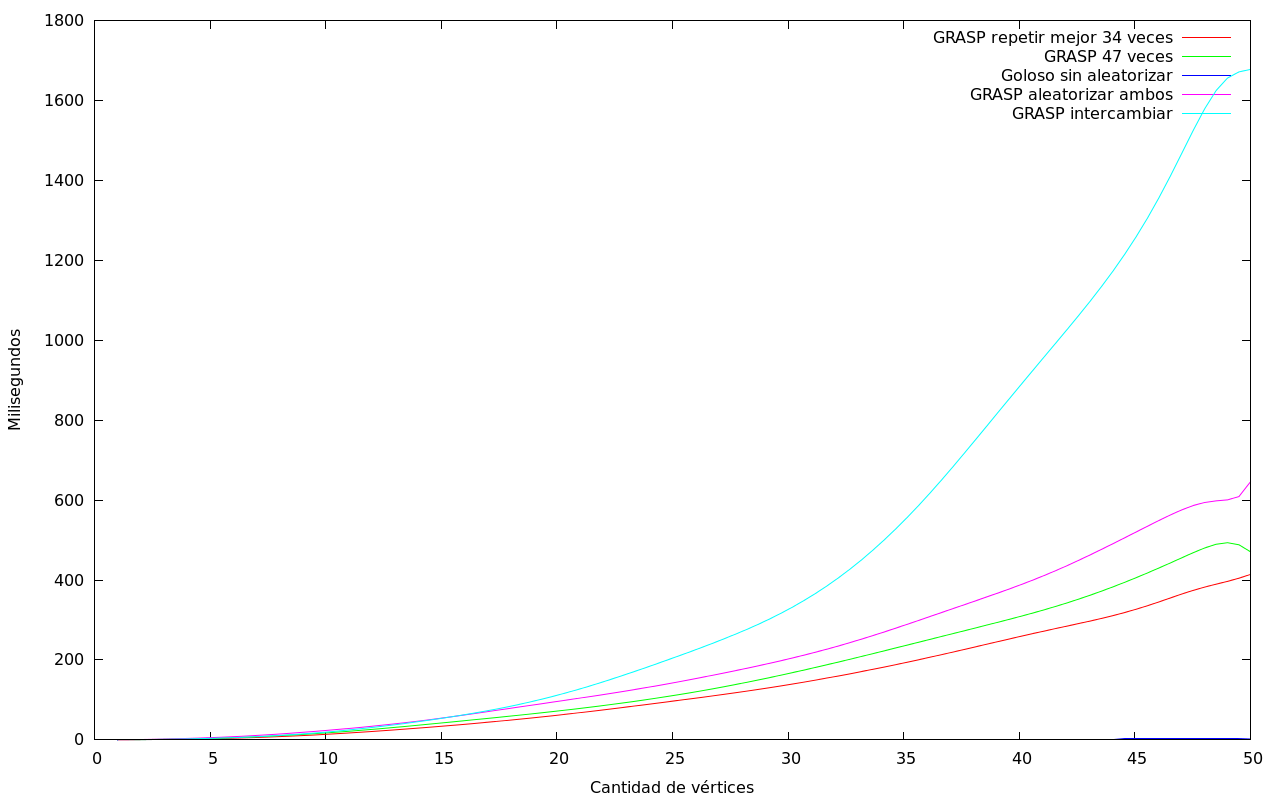
\includegraphics[scale=0.35]{imagenes/ej6-denso-pesos-distintos-k3-tiempo.png}
  \end{center}
\end{figure}

\vspace*{0.5cm}

Denso, aristas con pesos distintos, k=7
\vspace*{0.5cm}

\begin{figure}[h]
  \begin{center}
    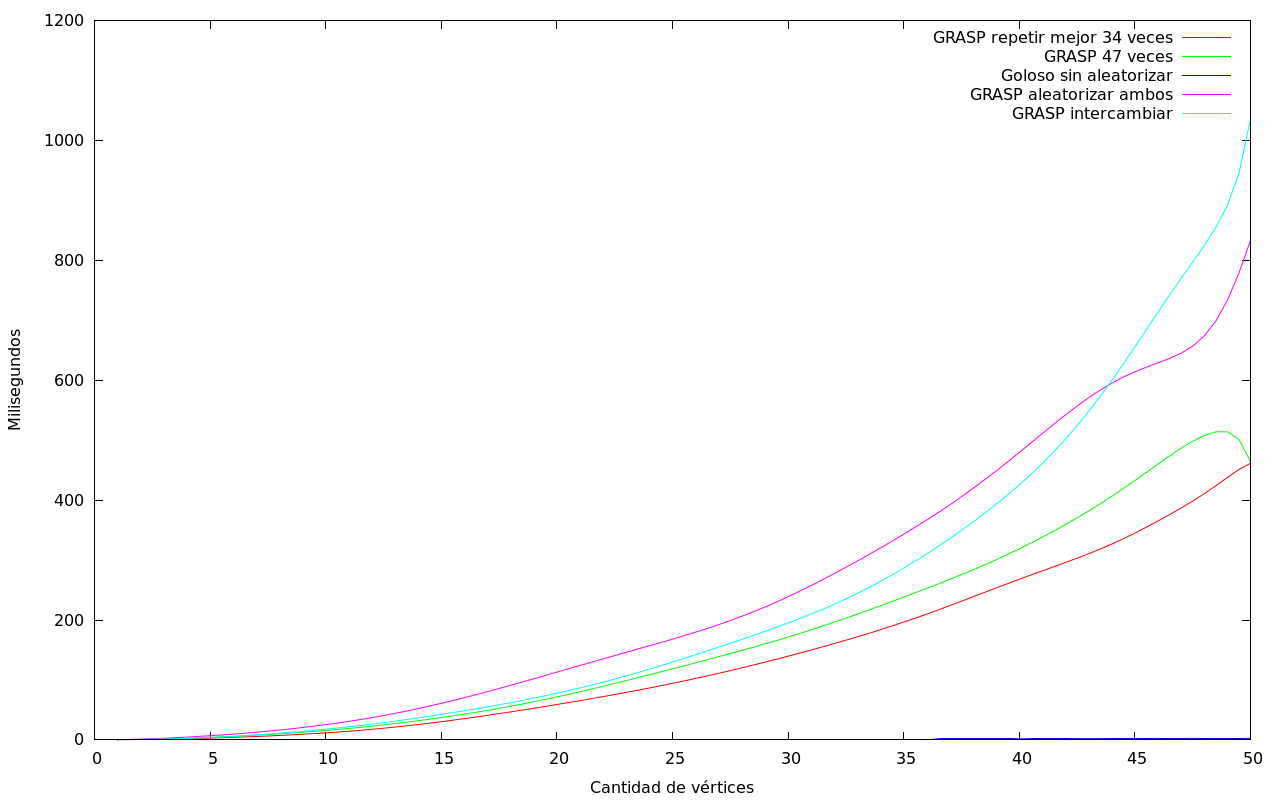
\includegraphics[scale=0.35]{imagenes/ej6-denso-pesos-distintos-k7-tiempo.png}
  \end{center}
\end{figure}

\vspace*{0.5cm}

Aunque es difícil de graficar bien, el exacto crece mucho más rápido que todos
los otros algoritmos.
Lo ejecutamos hasta n=18, pero para que se puedan ver el resto de las líneas,
a veces, lo cortamos incluso antes, como puede verse en el gráfico del grafo
Completo con $k = 7$.

Eso puede hacer aparentar, en algunos casos (como en el gráfico de Arbol con
$k = 3$), que el exacto crece más lento, pero en realidad es que si agregáramos
uno o más puntos, crecería tanto que el resto de las líneas parecerían rectas
sobre el 0.

Lo primero que se puede notar, es que el goloso sin aleatorizar es el más
rápido, algo completamente esperable, ya que se ejecuta sólamente una vez contra
la ejecución de la heurística local y repetida decenas de veces en el GRASP.

Luego, también se observa que el peor de los GRASP es que utiliza la heurística
local de $intercambiar$, seguido del algoritmo GRASP que aleatoriza tanto
aristas como conjuntos.

Los dos algoritmos elegidos son los que menor tiempo tardan (exceptuando el
goloso puro), con una pequeña ventaja el que realiza menos repeticiones.

Sin embargo, todavía falta contrastar la calidad de estos:

Arbol, k=3
\vspace*{0.5cm}

\begin{figure}[h]
  \begin{center}
    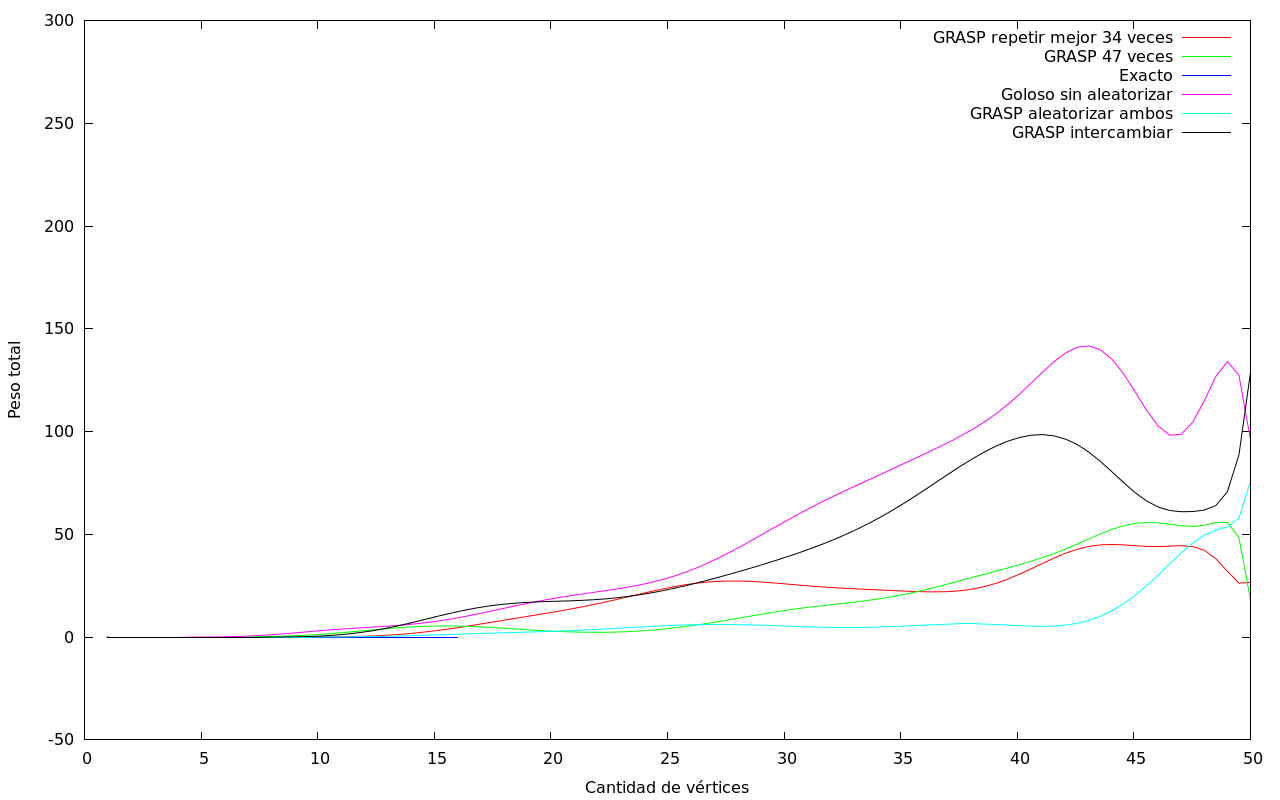
\includegraphics[scale=0.35]{imagenes/ej6-arbol-k3-peso.png}
  \end{center}
\end{figure}

\vspace*{0.5cm}

Completo, k=3
\vspace*{0.5cm}

\begin{figure}[h]
  \begin{center}
    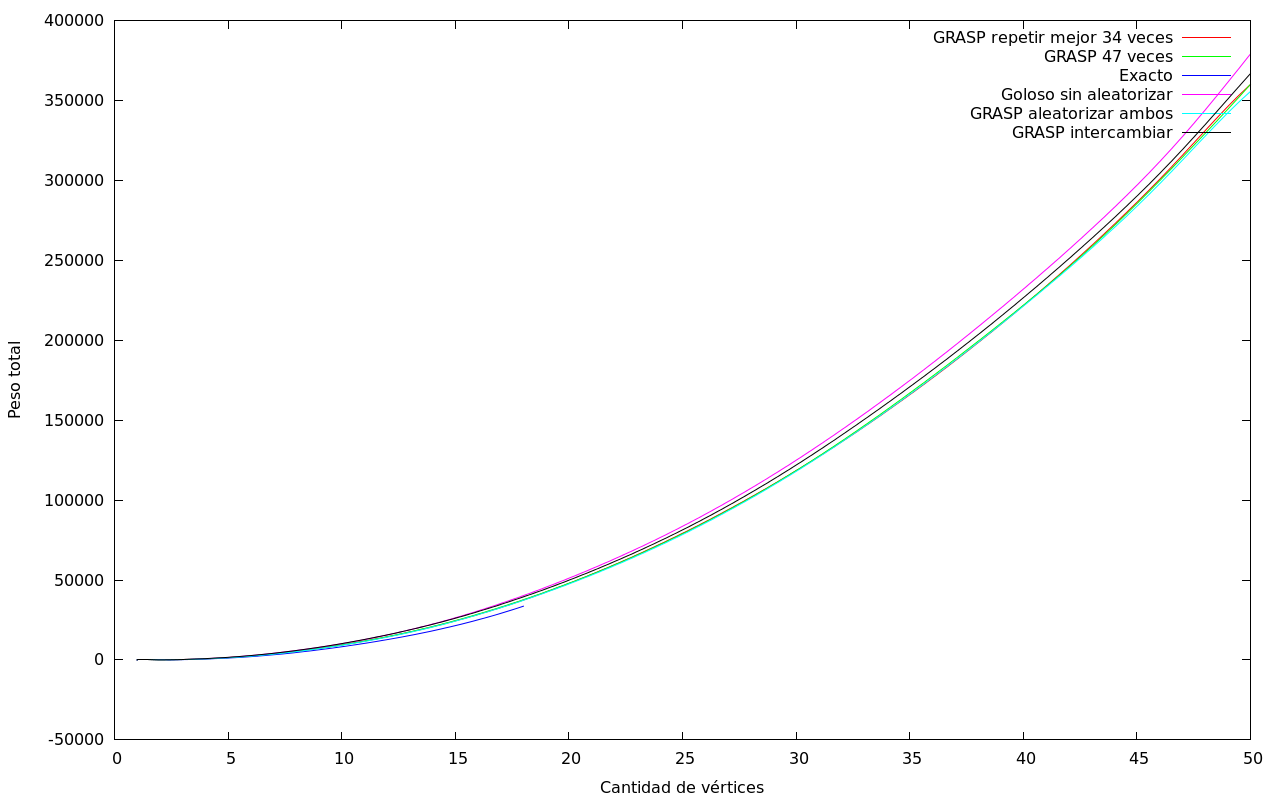
\includegraphics[scale=0.35]{imagenes/ej6-completo-k3-peso.png}
  \end{center}
\end{figure}

\vspace*{0.5cm}

Completo, k=7
\vspace*{0.5cm}

\begin{figure}[h]
  \begin{center}
    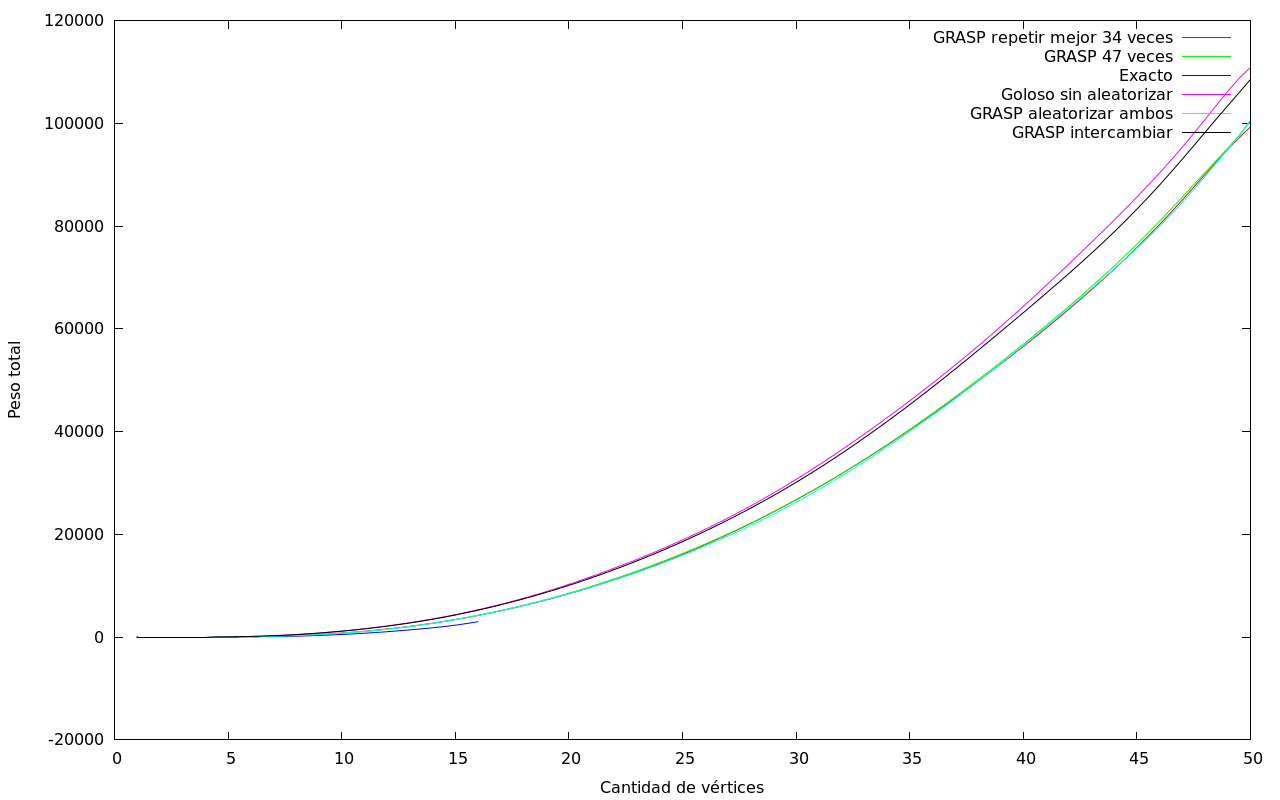
\includegraphics[scale=0.35]{imagenes/ej6-completo-k7-peso.png}
  \end{center}
\end{figure}

\vspace*{0.5cm}

Denso, aristas con pesos iguales, k=3
\vspace*{0.5cm}

\begin{figure}[h]
  \begin{center}
    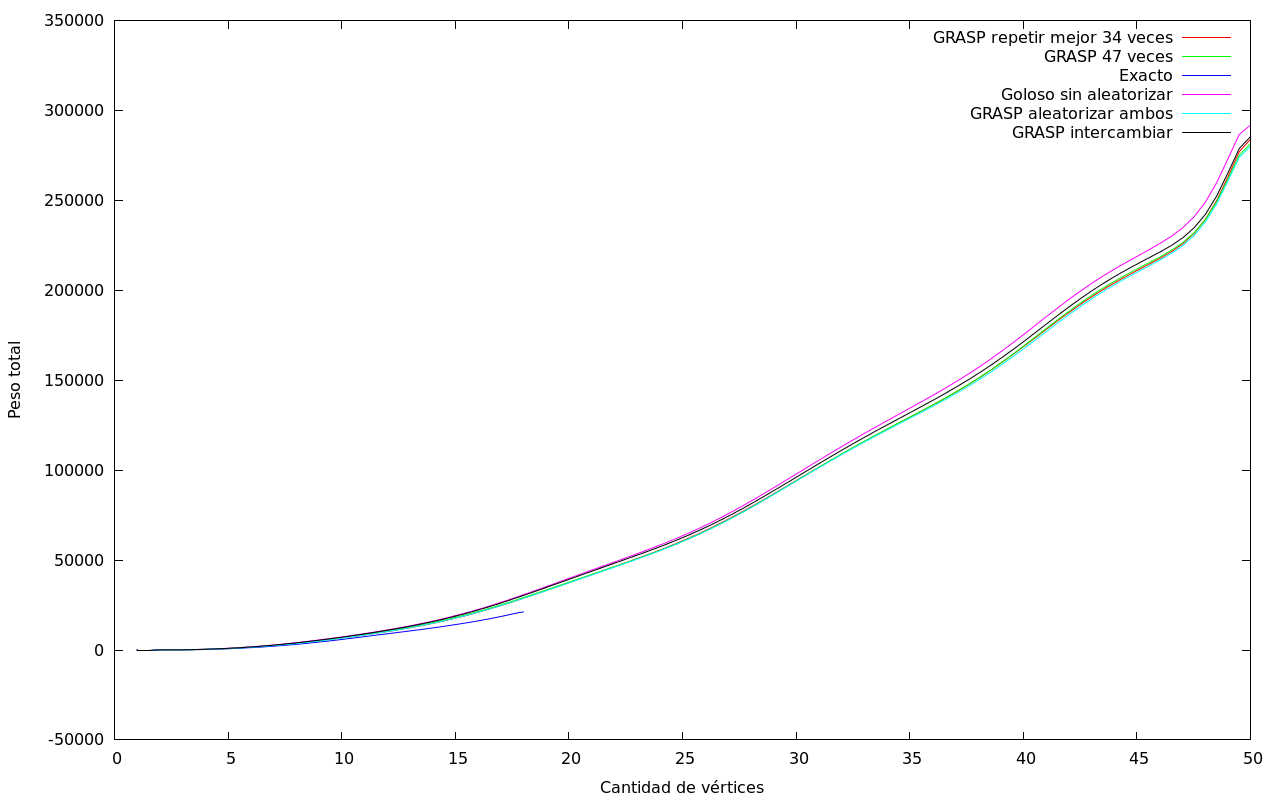
\includegraphics[scale=0.35]{imagenes/ej6-denso-pesos-iguales-k3-peso.png}
  \end{center}
\end{figure}

\vspace*{0.5cm}

Denso, aristas con pesos iguales, k=7
\vspace*{0.5cm}

\begin{figure}[h]
  \begin{center}
    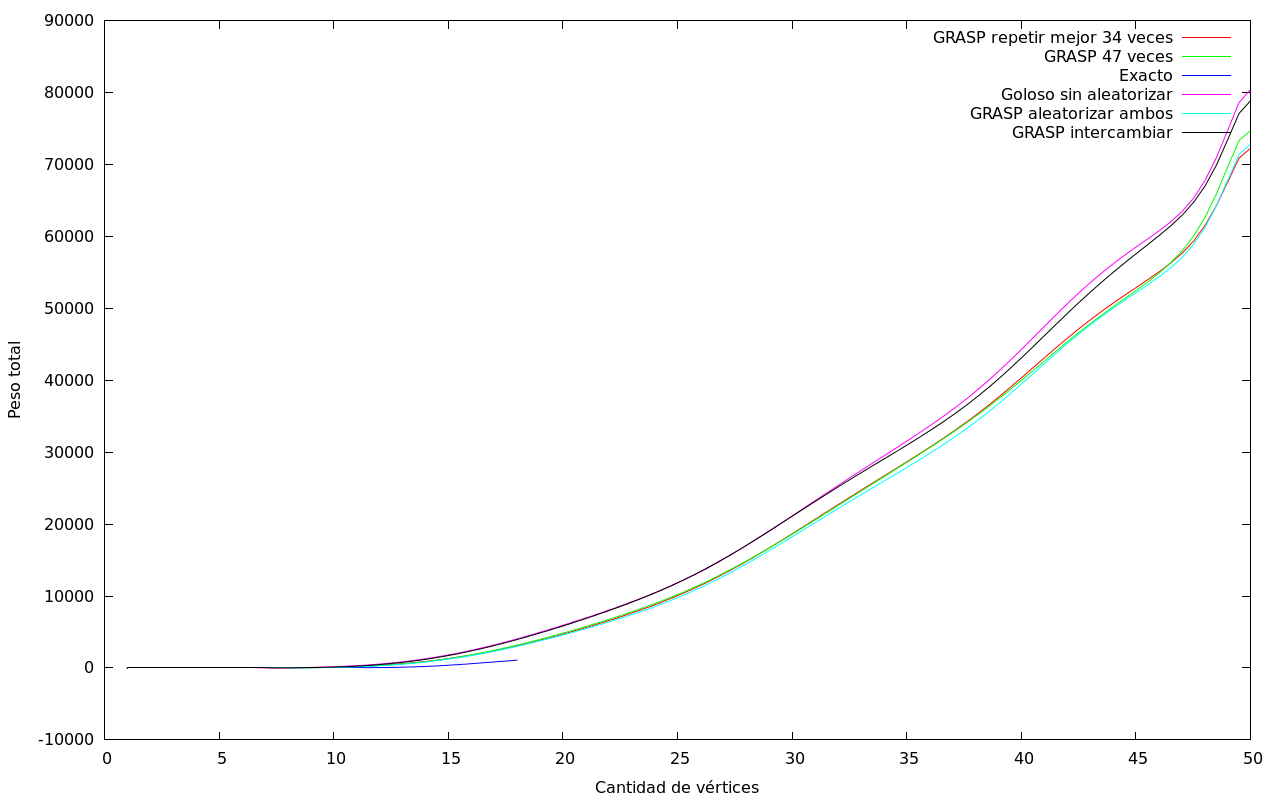
\includegraphics[scale=0.35]{imagenes/ej6-denso-pesos-iguales-k7-peso.png}
  \end{center}
\end{figure}

\vspace*{0.5cm}

Denso, aristas con pesos distintos, k=3
\vspace*{0.5cm}

\begin{figure}[h]
  \begin{center}
    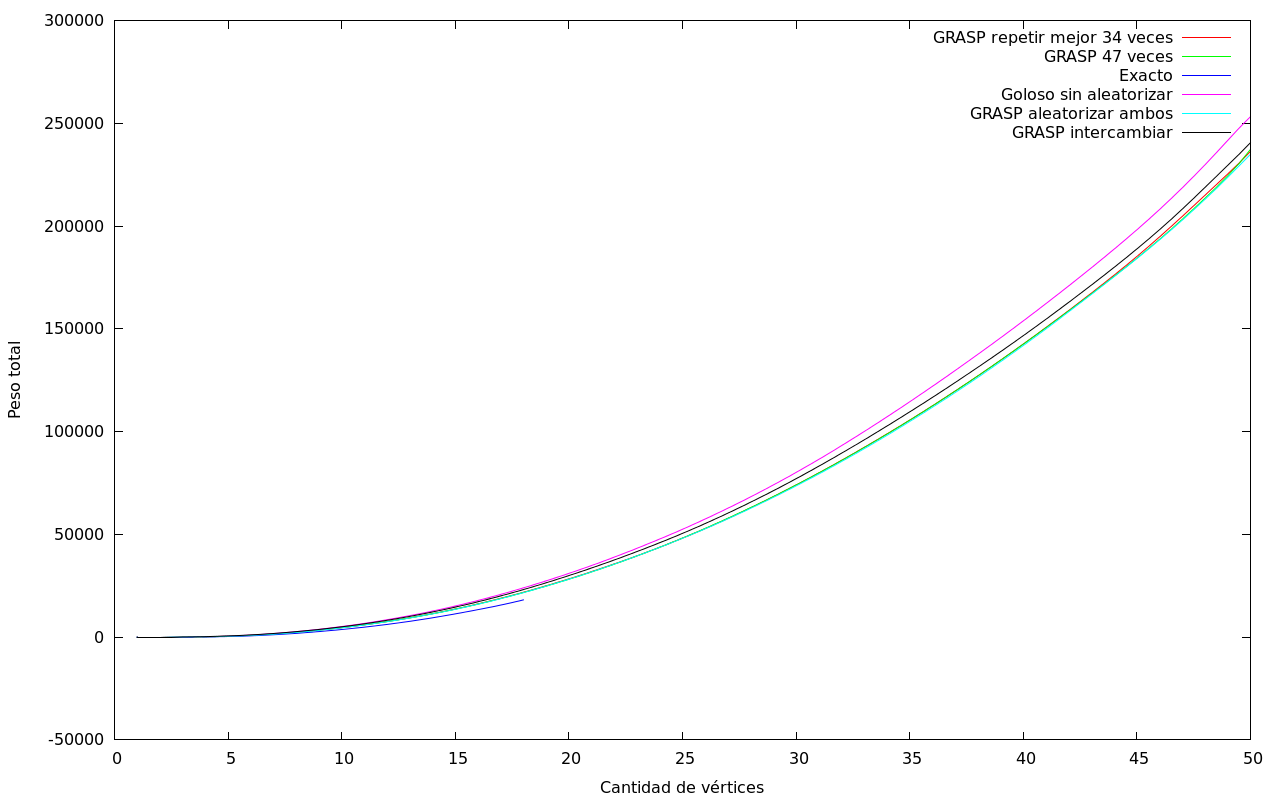
\includegraphics[scale=0.35]{imagenes/ej6-denso-pesos-distintos-k3-peso.png}
  \end{center}
\end{figure}

\vspace*{0.5cm}

Denso, aristas con pesos distintos, k=7
\vspace*{0.5cm}

\begin{figure}[h]
  \begin{center}
    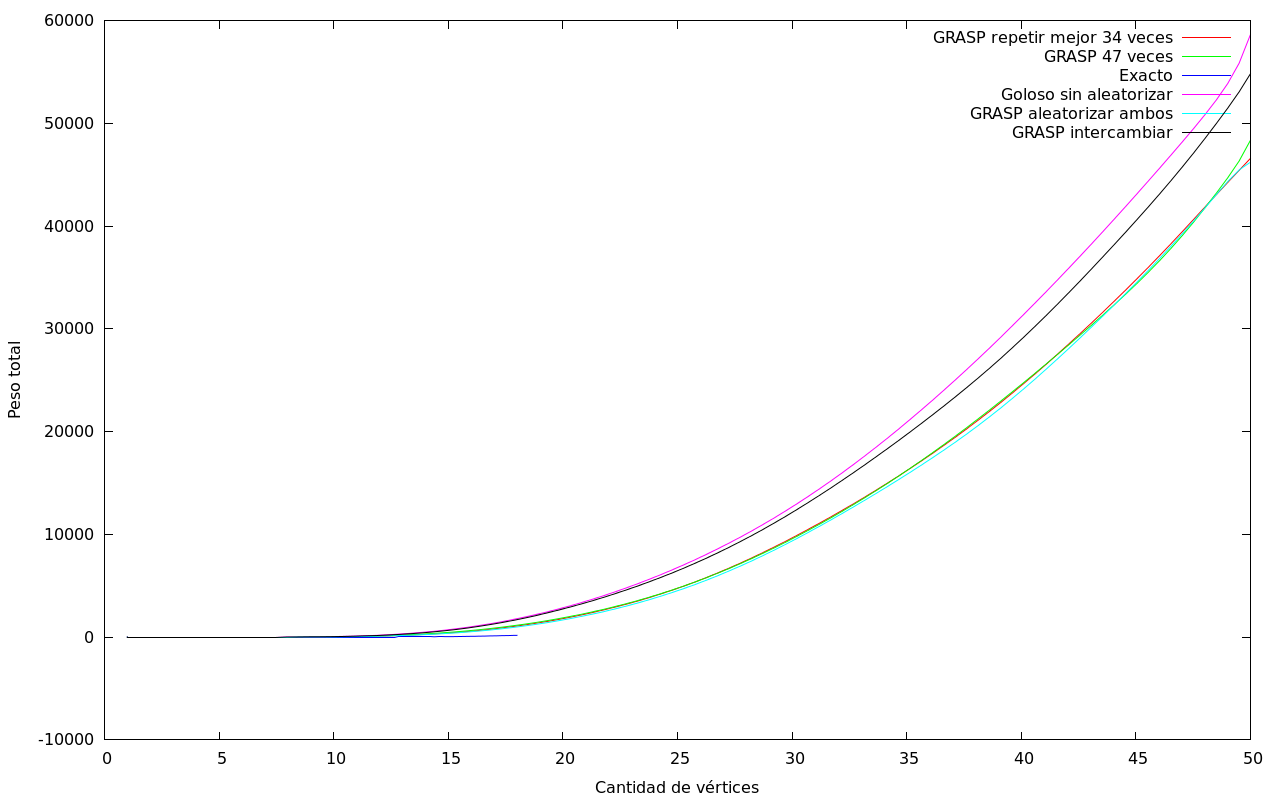
\includegraphics[scale=0.35]{imagenes/ej6-denso-pesos-distintos-k7-peso.png}
  \end{center}
\end{figure}

\vspace*{0.5cm}

Lo primero que podemos notar, es que en el árbol (un grafo bipartito, que puede
dividirse en 2 conjuntos y generar peso 0) y con $k = 3$, no todos llegan al
resultado obvio. Con $k = 7$ (no graficado) todos los algoritmos encuentran la
solución de peso 0.

Lo siguiente que se hace evidente, es que ninguno logra llegar al resultado
exacto (para $n > 10$) y, sin embargo, dan resultados bastante similares,
ninguno crece en mayor medida que los otros.

Finalmente, el peor de todos, igualmente, es el goloso sin aleatorizar,
seguido del GRASP que utiliza la heurística de búsqueda local de $intercambiar$.

Los otros tres algoritmos: los dos elegidos y el GRASP que aleatoriza aristas y
conjuntos, tienen resultados muy parecidos, con diferencias menores al 1\% y sin
que ninguno tenga peso inferior consistentemente sobre los otros dos.

Considerando que el que aleatoriza tanto aristas como conjuntos era más lento
que los otros dos, podemos confirmar que la elección hecha fue la correcta:

Utilizando la meta-heurísitica GRASP, aleatorizando la selección de aristas en
el algoritmo goloso, usando la vecindad $mover$ en el algoritmo de búsqueda
local y sin importar el criterio de terminación, pero dando un número
considerable de repeticiones (34 y 47), obtuvimos los mejores resultados en
todas las pruebas.

Sin embargo, no fueron lo suficientemente buenas como para dar el resultado
exacto (o bastante cercano), por lo que queda abierto a mejoras.

Otro dato interesante es que la heurística golosa sin aleatorizar, aunque es
definitivamente la de peor calidad, la diferencia de peso total no es tan grande,
pero si lo es la diferencia en tiempos de ejecución, hasta 3 órdenes de magnitud
más rápido para grafos densos.






% \newpage
% \section{Apéndice 1: acerca de los tests}
% \textcolor{red}{\textbf{completar!}}



% \newpage
% \section{Apéndice 2: secciones relevantes del código}
% \textcolor{red}{\textbf{completar!}}


\end{document}
